% !Mode:: "TeX:UTF-8"

\def\usewhat{pdflatex}                               % 定义编译方式 dvipdfmx 或者 pdflatex,默认为 dvipdfmx
                                                     % 方式编译,如果需要修改,只需改变花括号中的内容即可。
\documentclass[12pt,openany,oneside,ctexartutf8]{book}
                                                     % 本科生毕业论文通常采用单页排版
% !Mode:: "TeX:UTF-8"
%  Authors: 张井   Jing Zhang: prayever@gmail.com     天津大学2010级管理与经济学部信息管理与信息系统专业硕士生
%           余蓝涛 Lantao Yu: lantaoyu1991@gmail.com  天津大学2008级精密仪器与光电子工程学院测控技术与仪器专业本科生

%%%%%%%%%% Package %%%%%%%%%%%%
\usepackage{graphicx}                       % 支持插图处理
% \usepackage[a4paper,text={146.4true mm,239.2 true mm},top= 25.4true mm, bottom= 25.4true mm, left=31.7 true mm,head=6true mm,headsep=6.5true mm,foot=16.5true mm]{geometry}
\usepackage[a4paper,top=25.4mm, bottom=25.4mm, left=31.7mm, right=31.7mm, head=6true mm,headsep=6.5true mm,foot=17.5mm]{geometry}
                                            % 支持版面尺寸设置
\usepackage[squaren]{SIunits}               % 支持国际标准单位
\usepackage{float}
\usepackage{titlesec}                       % 控制标题的宏包
\usepackage{titletoc}                       % 控制目录的宏包
\usepackage{fancyhdr}                       % fancyhdr宏包 支持页眉和页脚的相关定义
\usepackage[UTF8]{ctex}                     % 支持中文显示
\usepackage{CJKpunct}
\usepackage{color}                          % 支持彩色
\usepackage{amsmath}                        % AMSLaTeX宏包 用来排出更加漂亮的公式
\usepackage{amssymb}                        % 数学符号生成命令
\usepackage[below]{placeins}    %允许上一个section的浮动图形出现在下一个section的开始部分,还提供\FloatBarrier命令,使所有未处理的浮动图形立即被处理
\usepackage{multirow}                       % 使用Multirow宏包,使得表格可以合并多个row格
\usepackage{booktabs}                       % 表格,横的粗线;\specialrule{1pt}{0pt}{0pt}
\usepackage{longtable}                      % 支持跨页的表格。
\usepackage{tabularx}                       % 自动设置表格的列宽
\usepackage{subfigure}                      % 支持子图 %centerlast 设置最后一行是否居中
\usepackage[subfigure]{ccaption}            % 支持子图的中文标题
\usepackage[sort&compress,numbers]{natbib}  % 支持引用缩写的宏包
\usepackage{enumitem}                       % 使用enumitem宏包,改变列表项的格式
\usepackage{calc}                           % 长度可以用+ - * / 进行计算
\usepackage{txfonts}                        % 字体宏包
\usepackage{bm}                             % 处理数学公式中的黑斜体的宏包
\usepackage[amsmath,thmmarks,hyperref]{ntheorem}  % 定理类环境宏包,其中 amsmath 选项用来兼容 AMS LaTeX 的宏包
\usepackage{CJKnumb}                        % 提供将阿拉伯数字转换成中文数字的命令
\usepackage{indentfirst}                    % 首行缩进宏包
\usepackage{CJKutf8}                        % 用在UTF8编码环境下,它可以自动调用CJK,同时针对UTF8编码作了设置

% \usepackage{fancybox} 

%\usepackage{hypbmsec}                      % 用来控制书签中标题显示内容
\newcommand{\tabincell}[2]{\begin{tabular}{@{}#1@{}}#2\end{tabular}}
\usepackage{xcolor}
%支持代码环境
\usepackage{listings}
\lstset{numbers=left,
language=[ANSI]{C},
numberstyle=\tiny,
extendedchars=false,
showstringspaces=false,
breakatwhitespace=false,
breaklines=true,
captionpos=b,
keywordstyle=\color{blue!70},
commentstyle=\color{red!50!green!50!blue!50},
frame=shadowbox,
rulesepcolor=\color{red!20!green!20!blue!20}
}
%支持算法环境
\usepackage[boxed,ruled,lined]{algorithm2e}
\usepackage{algorithmic}

\usepackage{array}
\newcommand{\PreserveBackslash}[1]{\let\temp=\\#1\let\\=\temp}
\newcolumntype{C}[1]{>{\PreserveBackslash\centering}p{#1}}
\newcolumntype{R}[1]{>{\PreserveBackslash\raggedleft}p{#1}}
\newcolumntype{L}[1]{>{\PreserveBackslash\raggedright}p{#1}}

% 生成有书签的 pdf 及其生成方式。通常可以在 tjumain.tex 文件的第一行选择 pdflatex 或者是 dvipdfmx 编译手段。如果选择前者,则使用 pdflatex + pdflatex 编译; 如果选择后者,在编译的时候选择 latex + bibtex + latex + latex 编译。出现混淆的时候,系统会报错。
% 如果您的pdf制作中文书签有乱码使用如下命令,就可以解决了
\def\atemp{pdflatex}\ifx\atemp\usewhat
\usepackage{cmap}                           % pdflatex 编译时,可以生成可复制、粘贴的中文 PDF 文档, 缺点是在Windows上显示时效果不大好,字体发虚
\usepackage{hyperref}
\hypersetup{
    unicode,
    pdfborder={0 0 0},
}
\fi
% \usepackage[pdftex,unicode,
%             CJKbookmarks=true,
%             bookmarksnumbered=true,
%             bookmarksopen=true,
%             colorlinks=false,
%             pdfborder={0 0 0},
%             citecolor=blue,
%             linkcolor=red,
%             anchorcolor=green,
%             urlcolor=blue,
%             breaklinks=true
%             ]{hyperref}

                                % 定义本文所使用宏包
\graphicspath{{figures/}}                            % 定义所有的 .eps 文件在 figures 子目录下
\begin{document}                                     % 开始全文
\begin{CJK*}{UTF8}{song}                             % 开始中文字体使用
	% !Mode:: "TeX:UTF-8"
%  Authors: 张井   Jing Zhang: prayever@gmail.com     天津大学2010级管理与经济学部信息管理与信息系统专业硕士生
%           余蓝涛 Lantao Yu: lantaoyu1991@gmail.com  天津大学2008级精密仪器与光电子工程学院测控技术与仪器专业本科生

% 2018/5/23修正
%           李幼萌 Youmeng Li: liyoumeng@tju.edu.cn   天津大学软件学院软件工程系

%%%%%%%%%%%%%%%%% Fonts Definition and Basics %%%%%%%%%%%%%%%%%
\newcommand{\song}{\CJKfamily{song}}    % 宋体
\newcommand{\fs}{\CJKfamily{fs}}        % 仿宋体
\newcommand{\kai}{\CJKfamily{kai}}      % 楷体
\newcommand{\hei}{\CJKfamily{hei}}      % 黑体
\newcommand{\li}{\CJKfamily{li}}        % 隶书
\newcommand{\yihao}{\fontsize{26pt}{26pt}\selectfont}       % 一号, 单倍行距
\newcommand{\xiaoyi}{\fontsize{24pt}{24pt}\selectfont}      % 小一, 单倍行距
\newcommand{\erhao}{\fontsize{22pt}{1.25\baselineskip}\selectfont}       % 二号, 1.25倍行距
\newcommand{\xiaoer}{\fontsize{18pt}{18pt}\selectfont}      % 小二, 单倍行距
\newcommand{\sanhao}{\fontsize{16pt}{16pt}\selectfont}      % 三号, 单倍行距
\newcommand{\xiaosan}{\fontsize{15pt}{15pt}\selectfont}     % 小三, 单倍行距
\newcommand{\sihao}{\fontsize{14pt}{14pt}\selectfont}       % 四号, 单倍行距
\newcommand{\xiaosi}{\fontsize{12pt}{12pt}\selectfont}      % 小四, 单倍行距
\newcommand{\wuhao}{\fontsize{10.5pt}{10.5pt}\selectfont}   % 五号, 单倍行距
\newcommand{\xiaowu}{\fontsize{9pt}{9pt}\selectfont}        % 小五, 单倍行距

\CJKtilde  % 重新定义了波浪符~的意义
\newcommand\prechaptername{第}
\newcommand\postchaptername{章}

\punctstyle{hangmobanjiao}             % 调整中文字符的表示,行内占一个字符宽度,行尾占半个字符宽度

% 调整罗列环境的布局
\setitemize{leftmargin=3em,itemsep=0em,partopsep=0em,parsep=0em,topsep=-0em}
\setenumerate{leftmargin=3em,itemsep=0em,partopsep=0em,parsep=0em,topsep=0em}

% 避免宏包 hyperref 和 arydshln 不兼容带来的目录链接失效的问题。
\def\temp{\relax}
\let\temp\addcontentsline
\gdef\addcontentsline{\phantomsection\temp}

% 自定义项目列表标签及格式 \begin{publist} 列表项 \end{publist}
\newcounter{pubctr} %自定义新计数器
\newenvironment{publist}{%%%%%定义新环境
\begin{list}{[\arabic{pubctr}]} %%标签格式
    {
     \usecounter{pubctr}
     \setlength{\leftmargin}{2.5em}   % 左边界 \leftmargin =\itemindent + \labelwidth + \labelsep
     \setlength{\itemindent}{0em}     % 标号缩进量
     \setlength{\labelsep}{1em}       % 标号和列表项之间的距离,默认0.5em
     \setlength{\rightmargin}{0em}    % 右边界
     \setlength{\topsep}{0ex}         % 列表到上下文的垂直距离
     \setlength{\parsep}{0ex}         % 段落间距
     \setlength{\itemsep}{0ex}        % 标签间距
     \setlength{\listparindent}{0pt}  % 段落缩进量
    }}
{\end{list}}

\makeatletter
\renewcommand\normalsize{
  \@setfontsize\normalsize{12pt}{12pt} % 小四对应 12 pt
  \setlength\abovedisplayskip{4pt}
  \setlength\abovedisplayshortskip{4pt}
  \setlength\belowdisplayskip{\abovedisplayskip}
  \setlength\belowdisplayshortskip{\abovedisplayshortskip}
  \let\@listi\@listI}
\def\defaultfont{\renewcommand{\baselinestretch}{1.63}\normalsize\selectfont} % 设置行距

\renewcommand{\CJKglue}{\hskip -0.1 pt plus 0.08\baselineskip} % 控制字间距,使每行 34 个汉字
\makeatother

%%%%%%%%%%%%% Contents %%%%%%%%%%%%%%%%%
\renewcommand{\contentsname}{目\qquad 录}
\setcounter{tocdepth}{1} % 控制目录深度
\titlecontents{chapter}[2em]{\vspace{.5\baselineskip}\xiaosan\song}
             {\prechaptername\CJKnumber{\thecontentslabel}\postchaptername\qquad}{}
             {\hspace{.5em}\titlerule*[10pt]{$\cdot$}\sihao\contentspage}
\titlecontents{section}[4.2em]{\vspace{.25\baselineskip}\sihao\song}
             {\thecontentslabel\quad}{}
             {\hspace{.5em}\titlerule*[10pt]{$\cdot$}\sihao\contentspage}
% \titlecontents{subsection}[4em]{\vspace{.25\baselineskip}\xiaosi\song}
%              {\thecontentslabel\quad}{}
%              {\hspace{.5em}\titlerule*[10pt]{$\cdot$}\sihao\contentspage}

%%%%%%%%%% Chapter and Section %%%%%%%%%%%%%
\setcounter{secnumdepth}{4}
\setlength{\parindent}{2em}

\renewcommand{\chaptername}{\prechaptername\CJKnumber{\thechapter}\postchaptername}
\titleformat{\chapter}{\centering}{\xiaosan\song}{\chaptername}{} %{2em}
\titlespacing{\chapter}{0pt}{0.1\baselineskip}{0.8\baselineskip}

\titleformat{\section}{\sihao\hei}{\thesection}{1em}{}
\titlespacing{\section}{0pt}{0.15\baselineskip}{0.25\baselineskip}

\titleformat{\subsection}{\sihao\hei}{\thesubsection}{1em}{}
\titlespacing{\subsection}{0pt}{0.1\baselineskip}{0.3\baselineskip}

\titleformat{\subsubsection}{\sihao\hei}{\thesubsubsection}{1em}{}
\titlespacing{\subsubsection}{0pt}{0.05\baselineskip}{0.1\baselineskip}

%%%%%%%%%% Table, Figure and Equation %%%%%%%%%%%%%%%%%
\renewcommand{\tablename}{表}                                     % 插表题头
\renewcommand{\figurename}{图}                                    % 插图题头
\renewcommand{\thefigure}{\arabic{chapter}-\arabic{figure}}       % 使图编号为 7-1 的格式 %\protect{~}
\renewcommand{\thesubfigure}{\alph{subfigure})}                   % 使子图编号为 a) 的格式
\renewcommand{\thesubtable}{(\alph{subtable})}                    % 使子表编号为 (a) 的格式
\renewcommand{\thetable}{\arabic{chapter}-\arabic{table}}         % 使表编号为 7-1 的格式
\renewcommand{\theequation}{\arabic{chapter}-\arabic{equation}}   % 使公式编号为 7-1 的格式

%%%%%% 定制浮动图形和表格标题样式 %%%%%%
\makeatletter
\long\def\@makecaption#1#2{
   \vskip\abovecaptionskip
   \sbox\@tempboxa{\centering\wuhao\song{#1\qquad #2} }
   \ifdim \wd\@tempboxa >\hsize
     \centering\wuhao\song{#1\qquad #2} \par
   \else
     \global \@minipagefalse
     \hb@xt@\hsize{\hfil\box\@tempboxa\hfil}
   \fi
   \vskip\belowcaptionskip}
\makeatother
\captiondelim{~~~~} %用来控制longtable表头分隔符

%%%%%%%%%% Theorem Environment %%%%%%%%%%%%%%%%%
\theoremstyle{plain}
\theorembodyfont{\song\rmfamily}
\theoremheaderfont{\hei\rmfamily}
\newtheorem{theorem}{定理~}[chapter]
\newtheorem{lemma}{引理~}[chapter]
\newtheorem{axiom}{公理~}[chapter]
\newtheorem{proposition}{命题~}[chapter]
\newtheorem{prop}{性质~}[chapter]
\newtheorem{corollary}{推论~}[chapter]
\newtheorem{definition}{定义~}[chapter]
\newtheorem{conjecture}{猜想~}[chapter]
\newtheorem{example}{例~}[chapter]
\newtheorem{remark}{注~}[chapter]
%\newtheorem{algorithm}{算法~}[chapter]
\newenvironment{proof}{\noindent{\hei 证明:}}{\hfill $ \square $ \vskip 4mm}
\theoremsymbol{$\square$}

%%%%%%%%%% Page: number, header and footer  %%%%%%%%%%%%%%%%%

%\frontmatter 或 \pagenumbering{roman}
%\mainmatter 或 \pagenumbering{arabic}
\makeatletter
\renewcommand\frontmatter{\clearpage
  \@mainmatterfalse
  }
\makeatother

%%%%%%%%%%%% References %%%%%%%%%%%%%%%%%
\renewcommand{\bibname}{参考文献}
% 重定义参考文献样式,来自thu
\makeatletter
\renewenvironment{thebibliography}[1]{
    \titleformat{\chapter}{\raggedright\sihao\hei}{\chaptername}{2em}{}
   \chapter*{\bibname}
   \wuhao
   \list{\@biblabel{\@arabic\c@enumiv}}
        {\renewcommand{\makelabel}[1]{##1\hfill}
         \settowidth\labelwidth{0 cm}
         \setlength{\labelsep}{0pt}
         \setlength{\itemindent}{0pt}
         \setlength{\leftmargin}{\labelwidth+\labelsep}
         \addtolength{\itemsep}{-0.7em}
         \usecounter{enumiv}
         \let\p@enumiv\@empty
         \renewcommand\theenumiv{\@arabic\c@enumiv}}
    \sloppy\frenchspacing
    \clubpenalty4000
    \@clubpenalty \clubpenalty
    \widowpenalty4000
    \interlinepenalty4000
    \sfcode`\.\@m}
   {\def\@noitemerr
     {\@latex@warning{Empty `thebibliography' environment}}
    \endlist\frenchspacing}
\makeatother

\addtolength{\bibsep}{-0.5em}     % 缩小参考文献间的垂直间距
\setlength{\bibhang}{2em}         % 每个条目自第二行起缩进的距离

% 参考文献引用作为上标出现
%\newcommand{\citeup}[1]{\textsuperscript{\cite{#1}}}
\makeatletter
    \def\@cite#1#2{\textsuperscript{[{#1\if@tempswa , #2\fi}]}}
\makeatother
%% 引用格式
\bibpunct{[}{]}{,}{s}{}{,}

%%%%%%%%%%%% Cover %%%%%%%%%%%%%%%%%
% 封面、摘要、版权、致谢格式定义
\makeatletter
\def\ctitle#1{\def\@ctitle{#1}}\def\@ctitle{}
\def\cdegree#1{\def\@cdegree{#1}}\def\@cdegree{}
\def\caffil#1{\def\@caffil{#1}}\def\@caffil{}
\def\csubject#1{\def\@csubject{#1}}\def\@csubject{}
\def\cgrade#1{\def\@cgrade{#1}}\def\@cgrade{}
\def\cauthor#1{\def\@cauthor{#1}}\def\@cauthor{}
\def\cnumber#1{\def\@cnumber{#1}}\def\@cnumber{}
\def\cstuid#1{\def\@cstuid{#1}}\def\@cstuid{}
\def\cdate#1{\def\@cdate{#1}}\def\@cdate{}
\long\def\cabstract#1{\long\def\@cabstract{#1}}\long\def\@cabstract{}
\long\def\eabstract#1{\long\def\@eabstract{#1}}\long\def\@eabstract{}
\def\ckeywords#1{\def\@ckeywords{#1}}\def\@ckeywords{}
\def\ekeywords#1{\def\@ekeywords{#1}}\def\@ekeywords{}
\def\cheading#1{\def\@cheading{#1}}\def\@cheading{}
\def\ccovertitle#1{\def\@ccovertitle{#1}}\def\@ccovertitle{}

\pagestyle{fancy}
  \fancyhf{}
  \fancyhead[C]{\song\wuhao \@cheading}  % 页眉显示天津大学 20XX 届本科生毕业论文
  \fancyfoot[C]{\song\xiaowu ~\thepage~}
\newlength{\@title@width}

% 定义封面
\def\makecover{
%\cleardoublepage%
   \phantomsection
    \pdfbookmark[-1]{\@ctitle}{ctitle}

    \begin{titlepage}
      \vspace*{10pt}
      \begin{center}

      \begin{figure}[h]
      \centering
      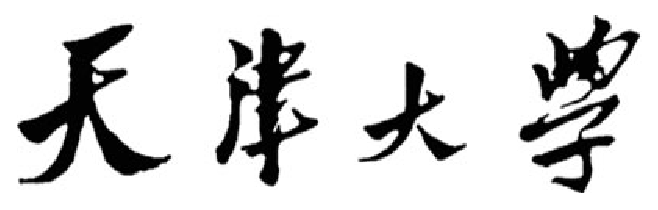
\includegraphics[width=0.4\textwidth]{figures/tju}
      \end{figure}
      \vspace*{15pt}
      \hei\erhao{\textbf{\@ccovertitle}} \\
      \hei\erhao{\textbf{\@ctitle}}
      \vspace*{55pt}

      \begin{figure}[h]
      \centering
      
\includegraphics[width=0.3\textwidth]{figures/Tjulogo}
      \end{figure}

      \vspace*{60pt}
      \renewcommand\arraystretch{1.5}
      \setlength{\@title@width}{5cm}
      {
        \sanhao\song{
          \begin{tabular}{lc}
            \textbf{学\qquad 院}  &  \underline{\makebox[\@title@width][c]{\textbf{\@caffil}}} \\
            \textbf{专\qquad 业}  &  \underline{\makebox[\@title@width][c]{\textbf{\@csubject}}} \\
            \textbf{年\qquad 级}  &  \underline{\makebox[\@title@width][c]{\textbf{\@cgrade}}}\\
            \textbf{姓\qquad 名}  &  \underline{\makebox[\@title@width][c]{\textbf{\@cauthor}}}\\
            \textbf{学\qquad 号}  &  \underline{\makebox[\@title@width][c]{\textbf{\@cstuid}}}\\
          \end{tabular}
        }
    }
    \vspace*{40pt}

    \song\sanhao{\textbf{\@cdate}}
    \end{center}
    \end{titlepage}
}

                             % 完成对论文各个部分格式的设置
	% !Mode:: "TeX:UTF-8"


%%%%%%%%%%%%%%%%%%%%%%%%%%%%%%%%%%%%%%%%%%%%%%%%%%%%%%%%%%%%%%%
%%  可通过对 setup/format.tex中                               %%
%%  第243行 \setlength{\@title@width}{5cm}中 5cm 这个参数来   %%
%%  控制封面中下划线的长度。                                   %%
%%%%%%%%%%%%%%%%%%%%%%%%%%%%%%%%%%%%%%%%%%%%%%%%%%%%%%%%%%%%%%

\cheading{天津大学软件学院~\the\year~年《专业课程设计2》结课报告}      % 正文页眉
\ccovertitle{《软件工程综合实践》结课报告}                       % 封面标题

%%%%%%%%%%%%%%%%%%%%%%%%%%%%%%%%%%%%%%%%%%%%%%%%%%%%%%%%%%%%%
%%%%%%%%%% 以下为论文的基本信息,需要由作者进行修改 %%%%%%%%%%%%
%%%%%%%%%%%%%%%%%%%%%%%%%%%%%%%%%%%%%%%%%%%%%%%%%%%%%%%%%%%%%
\ctitle{饿了吧项目实践报告}    % 封面用论文标题,自己可手动断行
\caffil{软件工程学院}       % 学院名称
\csubject{软件工程}     % 专业名称
\cgrade{2022级}           % 年级
\cauthor{杨宇鑫~谢帛洋}          % 学生姓名
\cstuid{~~~~3022207128~3022206049}     % 学号

\cdate{\the\year~年~\the\month~月~\the\day~日}  % 论文完成日期,不需要修改,自动生成

	\frontmatter                                     % 以下是论文导言部分,包括论文的封面,中英文摘要和中文目录
	\fancypagestyle{plain}{							 % 正文前均无页眉
		\fancyhf{}
		\renewcommand{\headrulewidth}{0 pt}
		\fancyfoot[C]{\song\xiaowu~\thepage~}
	}

	\makecover 			% 封面

	% !Mode:: "TeX:UTF-8"

% 目录
\defaultfont
\clearpage{
    \pagestyle{empty}
    \cleardoublepage
    \setcounter{page}{1}                                 % 单独从 1 开始编页码
    \pagenumbering{arabic}
    \titleformat{\chapter}{\centering\sanhao\hei}{\chaptername}{2em}{} % 设置目录两字的格式
    \pdfbookmark[0]{目~~录}{mulu}
    \tableofcontents                                     % 中文目录
    \thispagestyle{plain}
} % 目录

	\mainmatter\defaultfont\sloppy\raggedbottom
	\makeatletter
	\fancypagestyle{plain}{                              % 设置正文眉页脚风格
		\fancyhf{}
		\fancyhead[C]{\song\wuhao \@cheading}            % 页眉格式
		\fancyfoot[C]{\song\xiaowu ~\thepage~}           % 页脚格式
		\renewcommand{\headrulewidth}{0.5pt}
		\renewcommand{\footrulewidth}{0pt}
	}
	\makeatother
	\setcounter{page}{1}                                 % 单独从 1 开始编页码
	\titleformat{\chapter}{\centering\xiaosan\hei}{\chaptername}{2em}{} % 恢复chapter标题格式要求

	%%%%%% 这里是正文,每个文件对应正文中的一章 %%%%%%

	\chapter{软件需求规格说明书}
\section{引言}

\subsection{编写目的}

  
本文档的目的是详细地介绍饿了吧APP所包含的需求,以便客户能够知晓产品的确切需求以及开发人员能够根据需求进一步进行扩展开发,以下叙述将结合文字描述、数据流图、ER图等来描述饿了吧APP的功能、性能、用户界面、运行环境、外部接口以及针对用户操作给出的各种响应。本文档的预期读者有客户、开发人员等。

\subsection{背景}

  
该项目适用于喜欢吃餐厅菜肴但不喜欢出门或不善于做饭的各年龄段人群,由谢帛洋和杨宇鑫二人团队进行开发和部署。

\subsection{参考资料}

{[}1{]}窦万峰.软件工程方法与实践(第三版).北京:机械工业出版社,2016

{[}2{]}普莱斯曼.软件工程:实践者的研究方法(原书第8版).北京:机械工业出版社,2016

\section{任务概述}

\subsection{项目概述}


\subsubsection{项目简介}
  
饿了吧APP是一款针对各年龄段各类人群的外卖软件,大家可以在这里浏览各个餐厅的美食,以及足不出户享受菜肴。软件最大的特色是添加了AI智能咨询服务,输入需求就可以得到饮食建议,方便使用者进行选择。

\subsubsection{项目目标}

  
该项目的市场目标为以年轻人群体为主、外卖软件市场,应用目标为实现外卖以及饮食咨询工作。

\subsubsection{具体功能概述}


(1)搜索功能:通过餐厅名、餐品名或地址模糊搜索显示结果列表。

\begin{quote}
(2)点餐功能:进入餐厅后可以选择餐品加入购物车,点击购物车可以看到餐品明细,继而可以进行餐品支付。
\end{quote}

(3)咨询功能:可以询问智能AI得到推荐食谱。

(4)订单功能:可以显示未支付和已支付的所有订单,并能查看订单明细。

(5)我的信息:查看个人基本资料,可以进行个人资料的修改(包括电话、头像等)。

(6)商家功能:可以进行商家注册以及登录,登陆后可以上架商品,编辑商品信息等。

(7)点赞、收藏和评论功能:在商家列表页可以进行点赞、收藏以及评论功能。

\subsection{用户特点}

  本产品的用户主要是喜爱点外卖年轻人群体,接受新鲜事物的能力比较强,他们比较容易接受外卖菜肴。并且对于智能AI的认可度也比较高。尤其是当代有许多人比较`宅',这类人群是我们的重点目标客户。

\subsection{假定和约束}


(1)人力和时间的约束:本APP开发过程中需要考虑到人力和时间的约束,相较于一些软件的开发团队来说人员较少时间较短。

(2)技术发展的约束:计算机技术和发展的日新月异,将会给信息处理带来更多手段,同时也会带来更加丰富的信息表达形式,例如心形的人工智能等等,可能导致我们的搜索时候没有那么智能,这就要求软件在设计时要考虑技术变化的可能性,为可能的变化预留一定的处理能力。

\section{功能需求}

\subsection{功能划分}

1)饿了吧的顶层数据流图

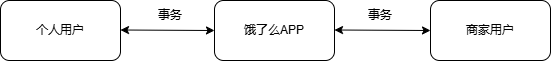
\includegraphics[width=5.73958in,height=0.63542in]{Picture30}

           图 1饿了么顶层数据流图

  
描述:如图1所示,用户可以扮演两种角色------个人用户、商家用户。当用户选择个人用户时,可以向饿了么发送事务(如修改资料等),同时个人用户可以浏览饿了么返回的事务,即个人用户与饿了么有双向的数据流动。当用户选择商家用户时,可以向饿了吧系统发送事务上架商品,同时可以浏览饿了吧返回的事务,即商家用户与饿了吧系统也有双向的数据流动。

(2)饿了吧的0层数据流图

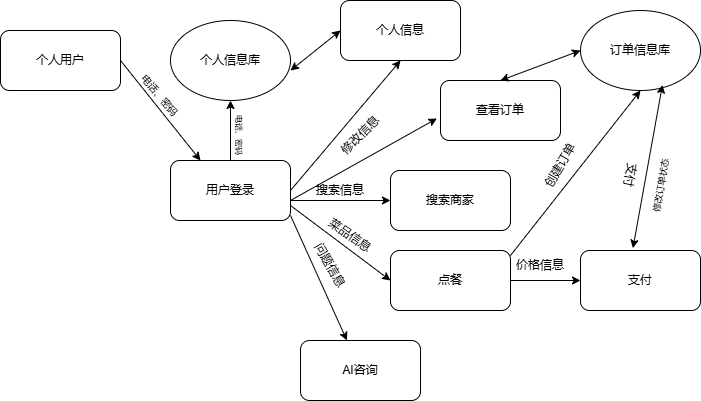
\includegraphics[width=5.76111in,height=3.29583in]{Picture31}

           图 2 饿了吧 0层数据流图

  
描述:如图2所示,个人用户通过提交身份信息向用户登录事务发送请求。用户登录事务从用户信息库中读取相应的用户信息进行匹配判断登录结果。用户登录成功后,用户可以进行个人信息管理、搜索商家、点餐、AI咨询、查看订单等操作。用户进行搜索操作时,用户提供的搜索信息流动到搜索事务,搜索事务对搜索信息进行相应的处理后得到商家信息。用户进行个人信息管理时,用户的修改信息传入信息修改事务中,修改个人信息库并返回修改后的新信息。进行点餐操作时发送菜品信息并进入支付事务,支付事务修改数据库创建新订单。其他操作同上述基本一致。

\subsection{功能描述}

(1)用户登录

​
功能描述:如图3所示,用户登录可以分为注册和登陆。注册时用户提供新用户注册信息发往注册事务,注册事务根据新用户注册信息得到新用户信息存入用户信息库,同时流动出用户信息。登录时用户提供用户名和密码发往登录事务,登录事务将得到的用户名和密码与用户信息库中的信息匹配,同时流动出用户信息。

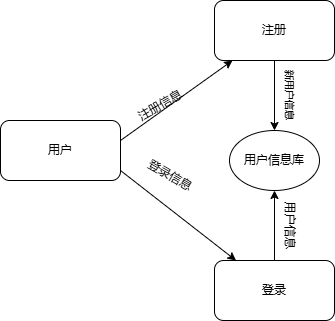
\includegraphics[width=2.94236in,height=2.81944in]{Picture32}

  图 3 用户登录功能细化数据流图

(2)个人信息管理

​
  功能描述:用户登录后可以进行相应操作进入个人信息管理界面,用户可以在此页面修改自己的个人信息。

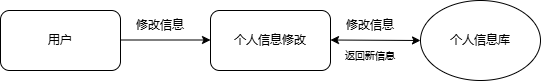
\includegraphics[width=5.63542in,height=0.84375in]{Picture33}

            图 4 个人信息管理功能细化数据流图

(3)搜索商家

​
功能描述:如图4所示,用户在搜索栏输入相应的搜索信息。搜索信息可以是商家名称或菜品名称。用户进入搜索商家事务,搜索商家事务处理传入的搜索信息流动出商家内容。

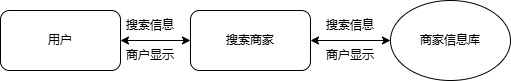
\includegraphics[width=5.32292in,height=0.84375in]{Picture34png}

           图 5 搜索功能细化数据流图

(4)点餐功能

​  
功能描述:用户选择菜品后提交菜品信息触发点餐事务,创建订单修改订单信息库,接着触发支付事务改变订单状态值。

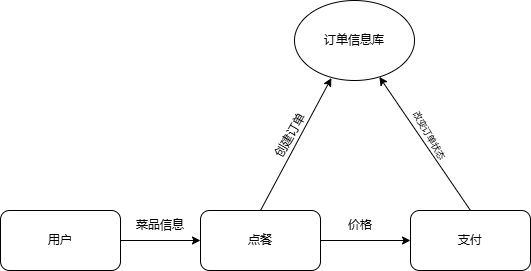
\includegraphics[width=4.22222in,height=2.15486in]{Picture35}

图 6 点餐功能细化数据流图

(5)咨询功能

​  功能描述:用户可以向智能AI传递问题信息,触发咨询事务,返回AI的回答。

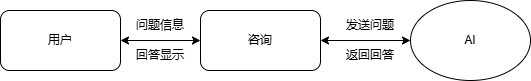
\includegraphics[width=5.53125in,height=0.84375in]{Picture36}

             图 7 咨询功能细化数据流图

(6)订单功能

  功能描述:用户点击订单后触发订单查看事务,事务从订单数据库查找订单数据并分为已支付和未支付,进行显示。

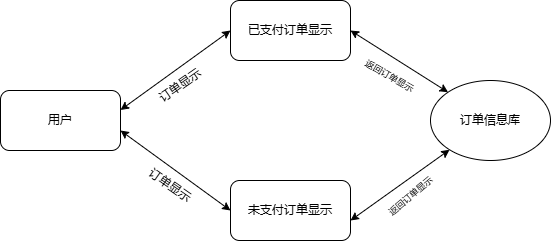
\includegraphics[width=5.17847in,height=2.26458in]{Picture37}

           图 8 订单功能细化数据流图

(7)点赞、评论和收藏功能

  功能描述:在商家列表处可以进行点赞、收藏、评论操作。点赞时用户触发点赞事务,向点赞信息库中加入信息,收藏同上。评论时用户触发评论事务,向评论信息库中加入信息,并且显示评论信息库中的每一条评论,即评论信息库向用户返回评论信息。

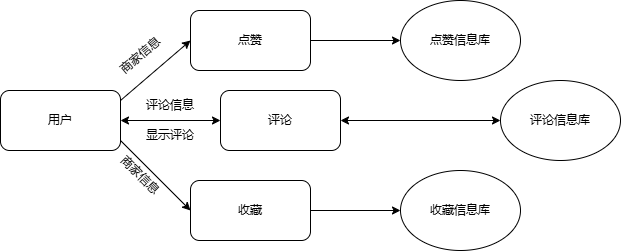
\includegraphics[width=5.76389in,height=2.32986in]{Picture38}

           图 9 点赞、评论和收藏功能细化数据流图

(8)商家功能

​  
功能描述:用户提交电话和密码触发商户登录事务,如果未进行注册则先进行注册事务,提交电话和密码至用户信息库。若进行过注册则进行比对,一致则登录成功。登陆事务出发后用户可以进行商户信息修改和上架商品等功能。

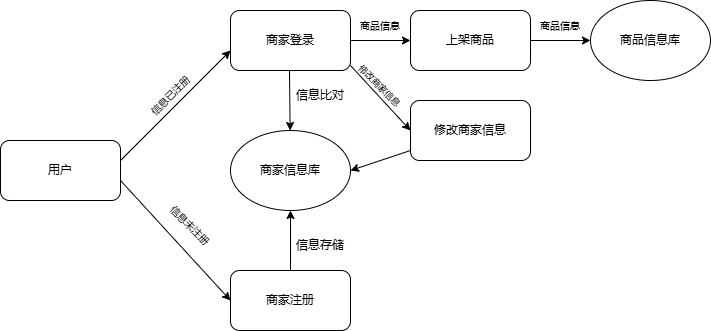
\includegraphics[width=5.76181in,height=2.68264in]{Picture39}

图 10 商家功能细化数据流图

\section{数据需求}

\subsection{静态数据}

用户信息、商户信息、点赞信息、收藏信息、评论信息、商品信息

\subsection{动态数据}

用户输入的搜索信息,输入框内的信息

\subsection{数据字典}

\section{数据流条目}

(1)身份信息

\begin{longtable}[]{@{}ll@{}}
\toprule
名称 & 身份信息\tabularnewline
简述 & 个人用户和商家用户的身份\tabularnewline
来源 & 个人用户和商家用户\tabularnewline
去处 & 用户登录\tabularnewline
\bottomrule
\end{longtable}

(2)用户名

\begin{longtable}[]{@{}ll@{}}
\toprule
名称 & 用户名\tabularnewline
简述 & 用户登录的账号\tabularnewline
类型 & varchar\tabularnewline
长度 & 1024\tabularnewline
来源 & 用户登录\tabularnewline
去处 & 用户信息库\tabularnewline
\bottomrule
\end{longtable}

(3)密码

\begin{longtable}[]{@{}ll@{}}
\toprule
名称 & 密码\tabularnewline
简述 & 用户登录的账号对应的密码\tabularnewline
类型 & varchar\tabularnewline
长度 & 1024\tabularnewline
来源 & 用户登录\tabularnewline
去处 & 用户信息库\tabularnewline
\bottomrule
\end{longtable}

(4)搜索商家

\begin{longtable}[]{@{}ll@{}}
\toprule
名称 & 搜索信息\tabularnewline
简述 & 用户发出搜索商户的信息\tabularnewline
来源 & 用户输入\tabularnewline
去处 & 搜索问题\tabularnewline
\bottomrule
\end{longtable}

(5)注册信息

\begin{longtable}[]{@{}ll@{}}
\toprule
名称 & 新用户注册信息\tabularnewline
简述 & 新用户进行注册的信息\tabularnewline
来源 & 用户输入\tabularnewline
去处 & 注册(用户信息库)\tabularnewline
\bottomrule
\end{longtable}

(6)点赞信息

\begin{longtable}[]{@{}ll@{}}
\toprule
名称 & 点赞信息\tabularnewline
简述 & 用户点赞时的信息\tabularnewline
来源 & 用户\tabularnewline
去处 & 点赞信息库\tabularnewline
\bottomrule
\end{longtable}

(7)收藏信息

\begin{longtable}[]{@{}ll@{}}
\toprule
名称 & 收藏信息\tabularnewline
简述 & 用户收藏时的信息\tabularnewline
来源 & 用户\tabularnewline
去处 & 收藏信息库\tabularnewline
\bottomrule
\end{longtable}

(8)评论信息

\begin{longtable}[]{@{}ll@{}}
\toprule
名称 & 评论信息\tabularnewline
简述 & 用户评论时的信息\tabularnewline
来源 & 用户输入\tabularnewline
去处 & 评论信息库\tabularnewline
\bottomrule
\end{longtable}

(9)商家列表

\begin{longtable}[]{@{}ll@{}}
\toprule
名称 & 商家列表\tabularnewline
简述 & 商家的信息列表\tabularnewline
来源 & 商家\tabularnewline
去处 & 查看商家\tabularnewline
\bottomrule
\end{longtable}

(10)商家信息

\begin{longtable}[]{@{}ll@{}}
\toprule
名称 & 商家信息\tabularnewline
简述 & 用户点单时展示的商家信息\tabularnewline
来源 & 商家\tabularnewline
去处 & 用户点单\tabularnewline
\bottomrule
\end{longtable}

(11)支付信息

\begin{longtable}[]{@{}ll@{}}
\toprule
名称 & 支付信息\tabularnewline
简述 & 进行支付时的信息\tabularnewline
来源 & 用户点单\tabularnewline
去处 & 用户支付\tabularnewline
\bottomrule
\end{longtable}

(12)订单信息

\begin{longtable}[]{@{}ll@{}}
\toprule
名称 & 订单信息\tabularnewline
简述 & 用户点单后产生的订单信息\tabularnewline
来源 & 用户点单\tabularnewline
去处 & 订单信息库\tabularnewline
\bottomrule
\end{longtable}

(13)AI咨询信息

\begin{longtable}[]{@{}ll@{}}
\toprule
名称 & AI咨询信息\tabularnewline
简述 & 用户输入的咨询问题\tabularnewline
来源 & 用户输入\tabularnewline
去处 & AI咨询\tabularnewline
\bottomrule
\end{longtable}

(14)个人信息

\begin{longtable}[]{@{}ll@{}}
\toprule
名称 & 个人信息\tabularnewline
简述 & 用户的个人信息展示\tabularnewline
来源 & 用户登录、用户信息库\tabularnewline
去处 & 我的信息功能\tabularnewline
\bottomrule
\end{longtable}

(15)修改的个人信息

\begin{longtable}[]{@{}ll@{}}
\toprule
名称 & 修改的个人信息\tabularnewline
简述 & 用户输入的新用户信息\tabularnewline
来源 & 我的信息中用户输入\tabularnewline
去处 & 我的信息功能\tabularnewline
\bottomrule
\end{longtable}

(16)商户用户名

\begin{longtable}[]{@{}ll@{}}
\toprule
名称 & 商户用户名\tabularnewline
简述 & 商户的电话号码\tabularnewline
来源 & 商户注册时的用户名\tabularnewline
去处 & 商户登录\tabularnewline
\bottomrule
\end{longtable}

(17)商户注册

\begin{longtable}[]{@{}ll@{}}
\toprule
名称 & 商户注册信息\tabularnewline
简述 & 商户注册时信息\tabularnewline
来源 & 商户输入\tabularnewline
去处 & 商户登录\tabularnewline
\bottomrule
\end{longtable}

(18)商户密码

\begin{longtable}[]{@{}ll@{}}
\toprule
名称 & 商户密码\tabularnewline
简述 & 商户登录的账号对应的密码\tabularnewline
类型 & varchar\tabularnewline
长度 & 1024\tabularnewline
来源 & 商户登录\tabularnewline
去处 & 商家信息库\tabularnewline
\bottomrule
\end{longtable}

(19)商品信息

\begin{longtable}[]{@{}ll@{}}
\toprule
名称 & 商品信息\tabularnewline
简述 & 商户商品的详细信息\tabularnewline
来源 & 商户\tabularnewline
去处 & 商品信息库\tabularnewline
\bottomrule
\end{longtable}

(20)上架商品信息

\begin{longtable}[]{@{}ll@{}}
\toprule
名称 & 上架商品信息\tabularnewline
简述 & 商户想要上架的商品信息\tabularnewline
来源 & 上架商品\tabularnewline
去处 & 商品信息库\tabularnewline
\bottomrule
\end{longtable}

(21)地址信息

\begin{longtable}[]{@{}ll@{}}
\toprule
名称 & 地址信息\tabularnewline
简述 & 外卖配送地址\tabularnewline
来源 & 地址添加\tabularnewline
去处 & 点餐功能\tabularnewline
\bottomrule
\end{longtable}

\section{数据存储条目}

(1)用户信息

\begin{longtable}[]{@{}ll@{}}
\toprule
名称 & 用户信息\tabularnewline
简述 & 描述用户的信息\tabularnewline
组成 & 用户名+密码+昵称+头像+Id\tabularnewline
组织方式 & 以Id为关键字\tabularnewline
\bottomrule
\end{longtable}

(2)地址信息

\begin{longtable}[]{@{}ll@{}}
\toprule
名称 & 地址信息\tabularnewline
简述 & 描述配送地址的信息\tabularnewline
组成 & 名称+电话+地址+编号\tabularnewline
组织方式 & 以编号为关键字\tabularnewline
\bottomrule
\end{longtable}

(3)商户信息

\begin{longtable}[]{@{}ll@{}}
\toprule
名称 & 用户信息\tabularnewline
简述 & 描述商家的信息\tabularnewline
组成 & 编号+图片+地址+类别+名称+商品+电话+密码\tabularnewline
组织方式 & 以编号为关键字\tabularnewline
\bottomrule
\end{longtable}

(4)商品信息

\begin{longtable}[]{@{}ll@{}}
\toprule
名称 & 商品信息\tabularnewline
简述 & 描述商品的信息\tabularnewline
组成 & 商品名称+编号+商户+图片\tabularnewline
组织方式 & 以编号为关键字\tabularnewline
\bottomrule
\end{longtable}

(5)点赞信息

\begin{longtable}[]{@{}ll@{}}
\toprule
名称 & 点赞信息\tabularnewline
简述 & 描述商家获得点赞的信息\tabularnewline
组成 & 用户编号+商家编号+点赞编号\tabularnewline
组织方式 & 以点赞编号为关键字\tabularnewline
\bottomrule
\end{longtable}

(6)收藏信息

\begin{longtable}[]{@{}ll@{}}
\toprule
名称 & 收藏信息\tabularnewline
简述 & 描述商家获得收藏的信息\tabularnewline
组成 & 用户编号+商家编号+收藏编号\tabularnewline
组织方式 & 以收藏编号为关键字\tabularnewline
\bottomrule
\end{longtable}

(7)评论信息

\begin{longtable}[]{@{}ll@{}}
\toprule
名称 & 评论信息\tabularnewline
简述 & 描述商家获得评论的信息\tabularnewline
组成 & 用户编号+商家编号+评论编号\tabularnewline
组织方式 & 以评论编号为关键字\tabularnewline
\bottomrule
\end{longtable}

\section{性能需求}

\subsection{数据精度}

\begin{longtable}[]{@{}lll@{}}
\toprule
字段 & 精度 & 备注\tabularnewline
用户名 & char型 & 符合中国大陆电话格式\tabularnewline
密码 & char型 & 8位以上,大小写、符号和数字都要包含\tabularnewline
昵称 & char型 & 8位以下\tabularnewline
用户是否存在 & map型 &
前端传过来含有用户名和密码的json对象,后端接受到之后在数据库中匹配,返回是否匹配的信息给前端\tabularnewline
用户ID & int型 & 自动赋值\tabularnewline
\bottomrule
\end{longtable}

\subsection{时间特性}

(1) 响应时间:用户任意操作后2秒内系统给予反馈信息。

(2) 更新处理时间:由系统运行状态来决定。

(3) 数据的转换和传送时间:能够在5秒内完成。

5.3 灵活性

  
当需求发生某些变化时,该软件的基本操作、数据结构、运行环境等等基本不会发生变化,只是对系统的数据库的文件和记录进行处理,就可以满足需求。

\section{运行需求}

\subsection{用户界面}


\begin{quote}
(1)注册:用户填写该页面的``用户名''、``昵称''、``密码''、``确认密码''、``头像''信息后点击提交即可成功注册,返回``注册是否成功的消息''。

(2)登录:用户填写该页面的``用户名''、``密码''信息后点击登录即可成功登录,如果用户没有账号可以点击下方按钮进行注册。

(3)主页:该页面展示各个不同种类的美食,底部显示主页、发现、订单、我的四个按钮,右上角显示登录注册按钮,可以进入不同的页面。

(4)个人中心:点击修改资料可以修改资料;中间提供展示该用户的基本数据信息;点击最下方的退出可以登出用户。

(5)点单流程:点击后展示每个类别的商家列表,再进一步点击可以展示商家的商品信息,并可以进行点单,进入支付页面并完成支付。

(6)AI咨询:点击首页发现键进入AI界面,可以输入想要咨询的问题并发送,返回的内容会被显示在下方。

(7)我的订单:订单界面分别显示已支付订单和未支付订单,并且可以点击下拉按钮显示订单明细,对于未支付订单可以点击去支付完成订单的支付。

(8)商户信息:进行商户登陆后会显示该商户的基本信息,如图片、名称以及电话和菜品等。

(9)上架商品:商家登陆后可以上架新商品,输入新商品的图片、价格、名称和简介即可上架。
\end{quote}

(10)搜索商户:用户可以在首页的搜索栏输入搜索内容,点击搜索后下方展示搜索出的商家,并可以点击商家进行点餐。

\subsection{软件接口}

1.操作系统:Microsoft Windows系统

2.软件设备:VScode、IntelliJ IDEA、MySQL8.0、eclipse

\subsection{质量属性}

1.可用性:用户可以使用

2.可靠性:在给定时间内可以满足无错运行的要求

3.可维护性:服务器重启、写进日志

4.安全性:对用户的密码加密

5.可移植性:移动端移植




	
\chapter{项目设计文档}

\section{数据库设计}

\subsection{business表}


\begin{longtable}[]{@{}lllll@{}}
\toprule
Field & Null & Key & Default & Extra\tabularnewline
businessId & NO & PRI & NULL & auto\_increment\tabularnewline
phoneNumber & NO & & NULL &\tabularnewline
password & NO & & NULL &\tabularnewline
businessName & NO & & 未命名商家 &\tabularnewline
businessAddress & YES & & NULL &\tabularnewline
businessExplain & YES & & NULL &\tabularnewline
businessImg & YES & & NULL &\tabularnewline
orderTypeId & YES & & NULL &\tabularnewline
starPrice & YES & & 0 &\tabularnewline
deliveryPrice & YES & & 0 &\tabularnewline
remarks & YES & & NULL &\tabularnewline
\bottomrule
\end{longtable}

\subsection{cart表}

\begin{longtable}[]{@{}llllll@{}}
\toprule
Field & Type & Null & Key & Default & Extra\tabularnewline
cartId & int & NO & PRI & NULL & auto\_increment\tabularnewline
foodId & int & NO & & NULL &\tabularnewline
businessId & int & NO & & NULL &\tabularnewline
userId & varchar(20) & NO & & NULL &\tabularnewline
quantity & int & NO & & NULL &\tabularnewline
\bottomrule
\end{longtable}

\subsection{chats表}

\begin{longtable}[]{@{}llllll@{}}
\toprule
Field & Type & Null & Key & Default & Extra\tabularnewline
currentUserId & varchar(50) & NO & & NULL &\tabularnewline
senderUserId & varchar(50) & NO & & NULL &\tabularnewline
receiverUserId & varchar(50) & NO & & NULL &\tabularnewline
message & varchar(255) & YES & & NULL &\tabularnewline
\bottomrule
\end{longtable}

\subsection{deliveryaddress表}

\begin{longtable}[]{@{}llllll@{}}
\toprule
Field & Type & Null & Key & Default & Extra\tabularnewline
daId & int & NO & PRI & NULL & auto\_increment\tabularnewline
contactName & varchar(20) & NO & & NULL &\tabularnewline
contactSex & int & NO & & NULL &\tabularnewline
contactTel & varchar(20) & NO & & NULL &\tabularnewline
address & varchar(100) & NO & & NULL &\tabularnewline
\bottomrule
\end{longtable}

\subsection{favorite表}

\begin{longtable}[]{@{}llllll@{}}
\toprule
Field & Type & Null & Key & Default & Extra\tabularnewline
userId & varchar(20) & NO & & NULL &\tabularnewline
businessId & int & NO & & NULL &\tabularnewline
\bottomrule
\end{longtable}

\subsection{food表}

\begin{longtable}[]{@{}llllll@{}}
\toprule
Field & Type & Null & Key & Default & Extra\tabularnewline
foodId & int & NO & PRI & NULL & auto\_increment\tabularnewline
foodName & varchar(30) & NO & & NULL &\tabularnewline
foodExplain & varchar(30) & NO & & NULL &\tabularnewline
foodImg & mediumtext & NO & & NULL &\tabularnewline
foodPrice & decimal(5,2) & NO & & NULL &\tabularnewline
businessId & int & NO & & NULL &\tabularnewline
remarks & varchar(40) & YES & & NULL &\tabularnewline
\bottomrule
\end{longtable}

\subsection{likes表}

\begin{longtable}[]{@{}llllll@{}}
\toprule
Field & Type & Null & Key & Default & Extra\tabularnewline
userId & varchar(20) & NO & PRI & NULL &\tabularnewline
businessId & int & NO & PRI & NULL &\tabularnewline
\bottomrule
\end{longtable}

\subsection{orderdetailet表}

\begin{longtable}[]{@{}llllll@{}}
\toprule
Field & Type & Null & Key & Default & Extra\tabularnewline
odId & int & NO & PRI & NULL & auto\_increment\tabularnewline
foodName & varchar(40) & YES & & NULL &\tabularnewline
orderId & int & NO & & NULL &\tabularnewline
foodId & int & NO & & NULL &\tabularnewline
quantity & int & NO & & NULL &\tabularnewline
priceAtThatTime & decimal(5,2) & NO & & 0 &\tabularnewline
\bottomrule
\end{longtable}

\subsection{orderdetailet food表} 

\begin{longtable}[]{@{}llllll@{}}
\toprule
Field & Type & Null & Key & Default & Extra\tabularnewline
odId & int & YES & & NULL &\tabularnewline
orderId & int & YES & & NULL &\tabularnewline
foodId & int & YES & & NULL &\tabularnewline
quantity & int & YES & & NULL &\tabularnewline
priceAtThatTime & decimal(5,2) & YES & & NULL &\tabularnewline
foodName & varchar(255) & YES & & NULL &\tabularnewline
foodExplain & varchar(255) & YES & & NULL &\tabularnewline
foodImg & varchar(255) & YES & & NULL &\tabularnewline
businessId & int & YES & & NULL &\tabularnewline
remarks & varchar(255) & YES & & NULL &\tabularnewline
\bottomrule
\end{longtable}

\subsection{orders表}

\begin{longtable}[]{@{}llllll@{}}
\toprule
Field & Type & Null & Key & Default & Extra\tabularnewline
orderId & int & NO & PRI & NULL & auto\_increment\tabularnewline
userId & varchar(20) & NO & & NULL &\tabularnewline
businessId & int & NO & & NULL &\tabularnewline
orderDate & date & YES & & NULL &\tabularnewline
orderTotal & decimal(7,2) unsigned zerofill & NO & & 0 &\tabularnewline
daId & int & YES & & NULL &\tabularnewline
orderState & int & NO & & 0 &\tabularnewline
\bottomrule
\end{longtable}

\subsection{remarks表}

\begin{longtable}[]{@{}llllll@{}}
\toprule
Field & Type & Null & Key & Default & Extra\tabularnewline
remark & varchar(255) & YES & & NULL &\tabularnewline
businessId & int & YES & & NULL &\tabularnewline
remarkDate & date & YES & & NULL &\tabularnewline
userId & varchar(20) & YES & & NULL &\tabularnewline
remarkId & int & NO & PRI & NULL & auto\_increment\tabularnewline
userName & varchar(20) & YES & & NULL &\tabularnewline
\bottomrule
\end{longtable}

\subsection{searchhistory表}

\begin{longtable}[]{@{}llllll@{}}
\toprule
Field & Type & Null & Key & Default & Extra\tabularnewline
userId & varchar(40) & NO & & NULL &\tabularnewline
searchContent & varchar(255) & NO & & NULL &\tabularnewline
\bottomrule
\end{longtable}

\subsection{user表}

\begin{longtable}[]{@{}llllll@{}}
\toprule
Field & Type & Null & Key & Default & Extra\tabularnewline
userId & varchar(20) & NO & PRI & NULL &\tabularnewline
password & varchar(20) & NO & & NULL &\tabularnewline
userName & varchar(20) & NO & MUL & NULL &\tabularnewline
userSex & int & NO & & 1 &\tabularnewline
userImg & mediumtext & YES & & NULL &\tabularnewline
delTag & int & NO & & 1 &\tabularnewline
\bottomrule
\end{longtable}


\section{前端设计}

\subsection{底部导航栏}
    


    首页:返回主界面。

    我的:包含用户的个人中心,如订单、收藏、账户设置等。

    发现:包含发现新商家或新活动的功能。

    订单:查看和管理用户的订单。
\subsection{首页}

    顶部导航栏:

    登录和注册按钮,允许用户进行账户管理。

    天津大学北洋园校区的下拉菜单,用于选择不同的校区或位置。

    搜索栏:

    提供搜索功能,用户可以搜索饿了么平台上的商家或商品名称。

    分类标签:

    早餐美食:可能包含早餐相关的食品选项。

    跑腿代购:提供代购服务,如汉堡披萨、甜品饮品等。

    速食简餐:快速方便的食品选择。

    地方小吃:提供地方特色小吃。

    米粉面馆:提供米粉、面条、包子、粥、炸鸡、炸串等食品。

    品质套餐:提供搭配齐全的套餐选项。

    促销活动:

    立即抢购:可能是限时抢购或特价活动的入口。

    超级会员:提供会员服务,每月享受超值权益。

    商家推荐:

    推荐商家列表,显示商家名称、评分、月销量、配送信息等。

    筛选和排序功能:

    筛选:允许用户根据综合排序、距离最近、销量最高等条件筛选商家。

    排序:提供排序功能,用户可以根据不同的标准对商家进行排序。

    商家详情:

    万家饺子(软件园E18店):显示商家的详细信息,包括评分、月销量、配送费用、起送价、配送距离和预计送达时间。

    蜂鸟专送:表明配送服务由蜂鸟专送提供。
\subsection{登录}

    密码输入区域:

    两个密码输入框,用于输入密码和确认密码。

    操作按钮:

    登录按钮:用于提交登录信息。

    去注册链接:引导新用户注册账户。
\subsection{商家列表} 

    标题:

    商家列表:标明这是商家列表的页面。

    商家信息:

    万家饺子(软件园E18店):商家名称,包括分店信息。

    商品种类:各种饺子,说明商家提供的主要商品。

    小锅饭豆腐馆(全运店):商家名称,包括分店信息。

    商品种类:小锅套餐,说明商家提供的主要商品。

    米村拌饭(浑南店):商家名称,包括分店信息。

    商品种类:拌饭、拌饭套餐、串,说明商家提供的主要商品。

    申记串道(中海康城店):商家名称,包括分店信息。

    商品种类:烤串、炸串,说明商家提供的主要商品。
    \subsection{商家信息}
 

    食品名称:食品的名称,包括烹饪方式。

    食品描述:描述食品的主要食材和特点。

    价格信息:食物的价格

    配送费用:另需配送费,说明除了食品价格外,还需要额外支付的费用。

    起送金额:标明用户下单的最低金额要求。
    \subsection{商单信息}

    订单标题:

    确认订单:标明这是用户需要确认的订单信息。

    配送信息:订单配送至:提示用户订单将被配送到的地址,具体的配送地址,收货人的联系电话。

    商家信息:订单来自的商家名称和分店信息。

    订单明细:用户所点的食品名称和数量,食品的价格,订单的配送费用。

    支付按钮:用户点击此按钮进行支付。

    订单总额:包括食品价格和配送费用的订单总金额。

    \subsection{支付信息}

    支付标题:

    在线支付:标明这是用户进行在线支付的页面。

    订单信息:

    订单信息:提示用户这是他们即将支付的订单详情。

    商家及订单金额:

    订单来自的商家名称和分店信息。

    订单的总金额,可能包括食品价格和配送费用。

    支付方式:

    支付宝:提供支付宝作为支付选项。

    微信支付:提供微信支付作为支付选项。

    支付按钮:用户点击此按钮以确认支付订单。
    \section{后端设计}
    
    \subsection{``我的''页面新增api}

    3.1.1.头像与昵称的获取接口:(原接口)

    UserController / getUserByIdByPass

    参数:userId、password

    返回值:user对象

    3.1.2.修改头像:(新增接口)

    UserController / changeUserAvatar

    参数:userId , base64 (头像的base64编码)

    返回值:int(影响的行数)

    3.1.3.修改昵称:(新增接口)

    UserController / changeUserName

    参数:userId , userName

    返回值:int (影响的行数)

    3.1.4.修改密码:(新增接口)

    UserController / changeUserPassword

    参数:userId , oldPassword , newPassword

    返回值:int (影响的行数)

    3.1.5 UserController/saveUser

    参数:userId , password , userName , userSex , userImg (可选)

    返回值:int (影响的行数)

    功能:向用户表中添加一条记录
    \subsection{评论和展示评论}

    3.2.1 RemarkController / listRemarksByBusinessId

    参数:businessId

    返回值:remark数组

    功能: 根据商家编号查询所属商家的所有评论信息

    3.2.2 RemarkController / saveRemarks

    参数:remark,userId,userName,businessId

    返回值:int (评论编号)

    功能:向评论表中添加一条记录,并返回评论编号

    3.2.3 RemarkController / removeOneRemark

    参数:userName userId businessId remark

    返回值:int 影响的行数

    功能:用户删除在某商家下的一条评论
    \subsection{收藏商家与展示收藏列表}

    3.3.1 FavoriteController / listFavoriteByUserId

    参数:userId

    返回值: businessId数组

    功能: 查询用户收藏的所有商家

    3.3.2 FavoriteController / saveFavoriteBusinessId

    参数:userId , businessId

    返回值:int (影响的行数)

    功能:当前用户收藏该商家(向收藏表中添加一条数据)

    3.3.3 FavoriteController / removeFavoriteBusinessId

    参数:userId , businessId

    返回值:int (影响的行数)

    功能:当前用户取消收藏该商家
    \subsection{点赞}

    3.4.1 LikesController / getLikesBybusinessId

    参数:businessId

    返回值: int (此商家的点赞总数量)

    功能: 查询某商家的点赞总数量

    3.4.2 LikesController / saveLikes

    参数:userId , businessId

    返回值:int (影响的行数)

    功能:用户点赞某一个商家

    3.4.3 LikesController / removeLikes

    参数:userId , businessId

    返回值:int (影响的行数)

    功能:用户取消点赞某一个商家

    3.4.4 LikesController / getLikesByUserIdByBusinessId

    参数:userId , businessId

    返回值:int (0:之前此用户对此商家未点赞

    1:之前此用户对此商家点过赞)

    功能:判断此用户对此商家之前有没有点过赞,

    若点过赞,则再点一次是取消点赞

    若未点过赞,则点一次是点赞
    \subsection{私信}

    3.5.1 ChatsController / removeChatsAllByCurrentUserId

    参数:currentUserId

    返回值:int (影响的行数)

    功能:清空当前用户的私信列表

    3.5.2 ChatsController / removeChatsByTwoUserIdByMessage

    参数:currentUserId , receiverUserId , message

    返回值:int (影响的行数)

    功能:删除当前用户currentUserId的与

    用户receiverUserId的内容为message的消息

    3.5.3 ChatsController / recallChatsByTwoUserIdByMessage

    参数:currentUserId , receiverUserId , message

    返回值:int (影响的行数)

    功能:撤回当前用户currentUserId的发送给

    用户receiverUserId的内容为message的消息

    3.5.4 ChatsController / getChatsByUserId

    参数:currentUserId

    返回值: chats数组

    功能: 查询当前用户的所有私信列表

    3.5.5 ChatsController / saveChats

    参数:senderUserId , receiverUserId , message

    返回值:int (影响的行数)

    功能:新增私信记录到总私信表中
    \subsection{商家登陆}

    3.6.1 BusinessController / saveBusiness

    参数:businessName ,password

    返回值:int (商家编号businessId)

    功能: 商家注册 并返回代表商家的唯一编号作为账号

    3.6.2 BusinessController / updateBusiness

    参数:businessId , businessAddress ,

    businessExplain , businessImg ,

    starPrice , deliveryPrice , orderTypeId

    返回值: int (影响的行数)

    功能:更改(完善)商家的信息

    3.6.3 FoodController / addFood

    参数:businessId , foodName , foodExplain ,

    foodImg , foodPrice

    返回值:int (食品的标号foodId)

    功能:商家可以上架自己的商品

    3.6.4 BusinessController / getBusinessByIdByPass

    参数:businessId , password

    返回值:int (影响的行数)

    功能:商家登录
    \subsection{搜索与搜索历史}

    3.7.1 SearchController / listBusiness

    参数:searchContent , userId (需要更新userId的这条历史搜索)

    返回值:business数组

    功能:根据关键词搜索商家列表

    3.7.2 SearchController / getHistoryByUserId

    参数:userId

    返回值:searchContent

    功能:查询用户上一次的一条搜索记录

    3.7.3 BusinessController / listBusinessByOrderTypeId

    参数:orderTypeId

    返回值:business数组

    功能:根据点餐分类编号查询所属商家信息

    3.7.4 BusinessController / getBusinessById

    参数:businessId

    返回值:business对象

    功能:根据商家编号查询商家信息

    3.7.5 RemarkController / listRemarksByBusinessId

    参数:businessId

    返回值:remark数组

    功能: 根据商家编号查询所属商家的所有评论信息
    \subsection{原项目基础API}

    \protect\hypertarget{2.3.1.business}{}{}3.8.1 business

    3.8.1.1 BusinessController/listBusinessByOrderTypeId

    参数:orderTypeId

    返回值:business数组

    功能:根据点餐分类编号查询所属商家信息

    3.8.1.2 BusinessController/getBusinessById

    参数:businessId

    返回值:business对象

    功能:根据商家编号查询商家信息

    \protect\hypertarget{2.3.2.food}{}{}3.8.2 food

    3.8.2.1. FoodController/listFoodByBusinessId

    参数:businessId返回值:food数组

    功能:根据商家编号查询所属食品信息

    \protect\hypertarget{2.3.3.cart}{}{}3.8.3 cart

    3.8.3.1 CartController/listCart

    参数:userId、businessId(可选)

    返回值:cart数组(多对一:所属商家信息、所属食品信息)功能:根据用户编号查询此用户所有购物车信息

    根据用户编号和商家编号,查询此用户购物车中某个商家的所有购物车信息

    3.8.3.2 CartController/saveCart

    参数:userId、businessId、foodId返回值:int(影响的行数)

    功能:向购物车表中添加一条记录

    3.8.3.3 CartController/updateCart

    参数:userId、businessId、foodId、quantity返回值:int(影响的行数)

    功能:根据用户编号、商家编号、食品编号更新数量

    3.8.3.4 CartController/removeCart

    参数:userId、businessId、foodId(可选)返回值:int(影响的行数)

    功能:根据用户编号、商家编号、食品编号删除购物车表中的一条食品记录根据用户编号、商家编号删除购物车表中的多条条记录

    \protect\hypertarget{2.3.4.deliveryAddress}{}{}3.8.4 deliveryAddress

    3.8.4.1 DeliveryAddressController/listDeliveryAddressByUserId

    参数:userId

    返回值:deliveryAddress数组

    功能:根据用户编号查询所属送货地址

    3.8.4.2 DeliveryAddressController/getDeliveryAddressById

    参数:daId

    返回值:deliveryAddress对象

    功能:根据送货地址编号查询送货地址

    3.8.4.3 DeliveryAddressController/saveDeliveryAddress

    参数:contactName、contactSex、contactTel、address、userId返回值:int(影响的行数)

    功能:向送货地址表中添加一条记录

    3.8.4.4 DeliveryAddressController/updateDeliveryAddress

    参数:daId、contactName、contactSex、contactTel、address、userId返回值:int(影响的行数)

    功能:根据送货地址编号更新送货地址信息

    3.8.4.5 DeliveryAddressController/removeDeliveryAddress

    参数:daId

    返回值:int(影响的行数)

    功能:根据送货地址编号删除一条记录

    \protect\hypertarget{2.3.5.orders}{}{}3.8.5 orders

    3.8.5.1 OrdersController/createOrders

    参数:userId、businessId、daId、orderTotal返回值:int(订单编号)

    功能:根据用户编号、商家编号、订单总金额、送货地址编号向订单表中添加一条记录,并获取自动生成的订单编号,

    然后根据用户编号、商家编号从购物车表中查询所有数据,批量添加到订单明细表中,然后根据用户编号、商家编号删除购物车表中的数据。

    3.8.5.2 OrdersController/getOrdersById

    参数:orderId

    返回值:orders对象(包括多对一:商家信息; 一对多:订单明细信息)

    功能:根据订单编号查询订单信息,包括所属商家信息,和此订单的所有订单明细信息

    3.8.5.3 OrdersController/listOrdersByUserId

    参数:userId

    返回值:orders数组(包括多对一:商家信息;
    一对多:订单明细信息)功能:根据用户编号查询此用户的所有订单信息

    新增:

    3.8.5.4.OrdersController / payOk

    参数:orderId

    返回值:int (影响的行数)

    功能:改变订单属性,将未支付0转成已支付1

    \protect\hypertarget{2.3.6.user}{}{}3.8.6 user

    3.8.6.1 UserController/getUserByIdByPass

    参数:userId、password返回值:user对象

    功能:根据用户编号与密码查询用户信息

    3.8.6.2 UserController/getUserById

    参数:userId

    返回值:int(返回行数)

    功能:根据用户编号查询用户表返回的行数


	
\chapter{项目测试文档}

\section{项目背景}

  饿了吧是一款面向各年龄段人群的外卖软件,让目标客户足不出户享受形形色色各个菜系的美食,并且让用户方便地了解不同商家的信息和菜品。
  \section{编写目的}
  

  该文档的目标人群是软件的开发团队以及使用软件的目标客户,以及软件的功能审核人员。给出测试方式和测试结果,方便审核人员对软件功能的进一步审核,也能够使用户对软件的功能更加了解。
  
  \section{测试人员}

  本次测试的主要人员是谢帛洋和杨宇鑫。

  \section{测试目标}
  在用使用软件之前,尽可能的发现软件中存在的错误和不合理之处,排除软件中存在的错和不合理之处,排出软件中潜在的错误,最终把高质量的软件系统交付给用户。系统的测试覆盖范围:功能、性能、UI、安全性、兼容性。

  \section{测试要求}

\begin{longtable}[]{@{}ll@{}}
\toprule
测试系统 & Windows11\tabularnewline
数据库版本 & Mysql 8.0\tabularnewline
其他 & VsCode、IDEA、Eclipse\tabularnewline
\bottomrule
\end{longtable}

\section{测试方法}

系统的功能测试选用了手工测试,运用黑盒测试中的等价类划分、边界值分析、错误推断、因果图法。

UI方面的测试包括:易用性测试、规范性测试、帮助设施测试、合理性测试、美观与协调性测试、独特
性测试、快捷方法组合组合测试。

系统的安全性、兼容性、配置测试也是手工测试

单元测试采用方法是白色测试,功能测试采用黑盒测试

\section{测试内容}


\subsection{单元测试}

首先依照系统、子系统和模块进行划分名单时最终的单元必须是功能模块,或者面向对象过程中的若干类,单元测试是对功能模块进行正确性验证的测试工作,也是后续测试的基础。目的在于发现各模块内部可能存在的各种差错,因此需要从程序内部结构出发设计测试用例,着重考虑以下五个方面:

模块接口:对所测模块的数据流进行测试。

局部数据结构:检查不正确不一致的数据类型说明、适用尚未赋值或者尚未初始化的变量、错误的初始值或者缺省值

路径:设计测试用例查找由于不正确计算(算法错、表达式的符号不正确、运算精度不够等)不正确的比较或者不正常的测试流(包括不同数据类型的相互比较、不适当地修改了循环变量、错误的或不可能的循环终止条件等)检查模块有没有对于常见的条件设计比较完善的错误处理功能,保证其逻辑上的正确性,注意设计数据流、控制流中刚好等于、大于或小于确定的比较直的用例。

\subsection{集成测试}

集成测试也叫组装测试、联合测试。通常在单元测试的基础上需要将所有的模块按照设计要求组装系统,这时需要考虑的问题如下:

(1)把各个模块连接起来,模块接口的数据是否会丢失

(2)一个模块的功能是否会对另一个模块的功能产生不利的影响

(3)全局数据结构是否有问题

(4)单元模块的误差积累起来,是否会放大,从而达到不能接受对策程度。我们在组装的时候可以参考采用一次性组装方式或者增值式组装方式

\subsection{系统测试}

(1)功能测试

验证系统功能是否符合其需求规格说明书,核实系统功能上是否完整,没有冗余和遗漏功能。详细介绍如下表:

\begin{longtable}[]{@{}ll@{}}
\toprule
测试范围 &
验证数据精确度、数据类型、业务功能等相关方面的正确性\tabularnewline
测试目标 & 核实所有功能均已正常实现、即是否与需求一致\tabularnewline
技术 & 采用黑盒测试、边界测试、等价类划分测试方法\tabularnewline
工具与方法 & 手工测试\tabularnewline
开始标准 & 开发阶段对应的功能完成并且测试用例设计完成\tabularnewline
完成标准 & 测试用例通过并且高级缺陷全部解决\tabularnewline
测试范围 &
验证数据精确度、数据类型、业务功能等相关方面的正确性\tabularnewline
\bottomrule
\end{longtable}


\subsection{用户界面测试}

  测试用户界面是否具有导航性、美观性、规范性、是否满足设计中客户要求的执行功能、详细介绍如下边UI测试:


\begin{longtable}[]{@{}ll@{}}
\toprule
测试范围 &
保证窗口运行、提示信息、页面跳转、易于使用等方面的正确性\tabularnewline
测试目标 &
核实各个窗口的风格(包括颜色、字体、提示信息、图标、title等)均与需求保持一致,或符合可接受标准,能够保证用户界面的友好性、易操作性、且符合用户操作习惯\tabularnewline
技术 & Web 测试通用方法\tabularnewline
工具与方法 & 手工测试、目测\tabularnewline
开始标准 & 界面开发完成\tabularnewline
完成标准 & UI
符合可接受标准,能保证用户界面的友好性,易操作性,而且符合用户操作习惯\tabularnewline
\bottomrule
\end{longtable}

\subsection{性能测试}

  测试相应时间、事务处理效率和其他时间敏感的问题。介绍如下表:


\begin{longtable}[]{@{}ll@{}}
\toprule
测试范围 & 多用户长时间在线操作时性能方面的测试\tabularnewline
测试目标 &
核实系统在大流量的数据与多用户操作时软件性能的稳定性,不造成系统崩溃或者相关\tabularnewline
技术 & 手动测试、自动化测试\tabularnewline
开始标准 & 系统测试\tabularnewline
完成标准 & 系统满足用户需求的性能要求\tabularnewline
\bottomrule
\end{longtable}

\subsection{兼容性测试}

  测试软件在不同平台上的使用的兼容性。介绍如下:

\begin{longtable}[]{@{}ll@{}}
\toprule
测试范围 & \vtop{\hbox{\strut 1.
使用不同版本的浏览器、分辨率、操作系统分别进行测试}\hbox{\strut 2.不同操作系统、不同设备、浏览器、分辨率等各种条件的组合测试}}\tabularnewline
测试目标 & 核实系统在不同软件和硬件配置中运行稳定\tabularnewline
技术 & 黑盒测试\tabularnewline
& 手工测试\tabularnewline
开始标准 & 系统测试\tabularnewline
完成标准 &
在各种不同版本不同类型浏览器、操作系统或者其组合下均能正常实现其功能(测试根据开发提供的依据决定测试的范围)\tabularnewline
\bottomrule
\end{longtable}

\subsection{安全性测试}

\begin{longtable}[]{@{}ll@{}}
\toprule
测试范围 & 用户、管理员的密码安全、权限\tabularnewline
测试目标 &
用户、管理员密码管理、应用程序级别的安全性、核实用户只能操作其所有权限操作的功能;系统级别的安全性\tabularnewline
技术 & 黑盒测试\tabularnewline
工具与方法 & 手工测试\tabularnewline
开始标准 & 系统测试\tabularnewline
\bottomrule
\end{longtable}

\subsection{配置测试}

  测试在不同网络、服务器、工作站的不同软硬件配置条件下,软件系统的质量,详细说明见下表:

\begin{longtable}[]{@{}ll@{}}
\toprule
测试范围 & 不同网络、服务器、不同软硬件配置条件\tabularnewline
测试目标 &
核实系统在不同的软硬件配置条件下系统的质量是否达到标准\tabularnewline
技术 & 黑盒测试\tabularnewline
工具与方法 & 手工测试\tabularnewline
开始标准 & 系统开发完成后\tabularnewline
完成标准 & 达到相关要求\tabularnewline
测试重点与优先级 & 测试优先级以测试需求优先级为参照\tabularnewline
需考虑的特殊事项 & 软硬件设备问题\tabularnewline
\bottomrule
\end{longtable}

\subsection{回归测试}

\begin{longtable}[]{@{}ll@{}}
\toprule
测试范围 & 所有功能、用户界面、兼容性、安全性等测试类型\tabularnewline
测试目标 &
核实执行所有测试类型后功能、性能、等均达到用户需求所要求的标准\tabularnewline
技术 & 黑盒测试\tabularnewline
工具与方法 & 手工测试 、 自动化测试\tabularnewline
开始标准 &
每当被测试的软件或其开发环境改变时,在每个核实的测试阶段上进行回归测试\tabularnewline
完成标准 & 95\% 的测试用例执行通过并通过系统测试\tabularnewline
测试重点与优先级 & 测试优先级以测试需求的优先级为参照\tabularnewline
需考虑的特殊事项 & 软硬件设备问题\tabularnewline
\bottomrule
\end{longtable}

\section{测试结果}

\subsection{测试中存在的问题}

\subsubsection{AI咨询功能在前端显示时会出现无返回结果的问题}

\subsubsection{修改头像约有10\%的数据传不到数据库}


\subsection{项目评价}


  在测试的过程中,测试团队并没有发现较大的bug,所述功能均可以基本实现,包括用户注册、登录以及基本的点餐流程、修改个人资料等功能。并且网页前端设计简洁清晰,对用户的引导性强,同时兼具了一定的美观性考量。
\section{测试用例}

	
\chapter{部署文档}

\section{项目背景}

\subsection{市场需求分析}
随着互联网技术的飞速发展和人们生活节奏的加快,外卖订餐服务已成为现代都市生活中不可或缺的一部分。越来越多的人选择通过手机应用程序或网站来订购美食,享受便捷的送餐服务。据统计,近年来外卖市场呈现出快速增长的趋势,市场规模不断扩大,用户数量持续攀升。因此,开发一款高质量的在线订餐平台具有巨大的市场需求和发展潜力。

\subsection{用户痛点分析}
尽管市场上已经存在多家知名的外卖平台,但在实际使用过程中,用户仍然面临诸多不便:
\subsubsection{选择困难}
面对众多的餐厅选项,用户往往难以快速做出决策。
\subsubsection{配送延迟}
高峰时段订单量大,导致配送时间延长,影响用餐体验。
\subsubsection{食品安全}
部分小餐馆卫生条件差,食品质量难以保证。
\subsubsection{个性化推荐不足}
现有的推荐算法不够精准,无法满足用户的个性化需求。

\subsection{商家需求分析}
对于餐饮商家而言,加入一个高效的外卖平台同样具有重要意义:
\subsubsection{拓宽销售渠道}
通过线上平台吸引更多的顾客,提高销售额。
\subsubsection{降低运营成本}
减少线下宣传费用,利用平台流量优势增加曝光度。
\subsubsection{提升服务质量}
借助平台提供的数据分析工具,优化菜品结构和服务流程。

\subsection{项目目标}
基于以上分析,“饿了吧”项目旨在打造一个高效、便捷且安全的在线订餐平台,具体目标包括:
\subsubsection{丰富菜品选择}
整合周边优质餐厅资源,提供多样化的菜品供用户选择。
\subsubsection{优化配送流程}
引入先进的物流管理系统,缩短配送时间,提升用户体验。
\subsubsection{保障食品安全}
严格筛选合作商家,确保所有上线餐厅均符合卫生标准。
\subsubsection{智能推荐系统}
利用大数据分析技术,根据用户喜好和历史订单记录进行个性化推荐。

通过实现这些目标,“饿了吧”项目将为用户提供更加优质的订餐体验,同时也为商家带来更多的商业机会,实现双赢的局面。


\section{系统需求}



\section{项目部署的系统需求}

\subsection{前端系统需求}
\subsubsection{操作系统}
- 支持主流的操作系统,包括 Windows、macOS 和 Linux。

\subsubsection{浏览器兼容性}
- 支持最新版本的 Chrome、Firefox、Safari 和 Edge 浏览器。

\subsubsection{移动设备}
- 支持 iOS 和 Android 操作系统的移动设备。

\subsection{后端系统需求}
\subsubsection{服务器配置}
- CPU:至少 2 核心

- 内存:至少 2 GB

- 硬盘:至少 5 GB 可用空间

\subsubsection{数据库}
- MySQL 5.7 或更高版本

\subsubsection{中间件}
- Nginx 作为反向代理服务器

- Redis 用于缓存和会话管理

- RabbitMQ 用于消息队列

\subsubsection{其他依赖}
- Java 8 或更高版本

- Spring Boot

- Maven

\subsection{网络需求}

\subsubsection{IP 地址}
- 具备公网 IP 地址,以便外部访问。

\subsection{安全性需求}
\subsubsection{数据加密}
- 使用 HTTPS 协议,确保数据传输的安全性。

\subsection{运维需求}

\subsubsection{持续集成/持续部署 (CI/CD)}
- 使用 宝塔面板 实现构建、测试和部署流程。

\subsubsection{日志管理}
- 收集和分析系统日志,快速定位问题。


\section{配置说明}

\subsection{数据库配置}

\subsubsection{数据库类型}
- MySQL

\subsubsection{数据库连接信息}
- 主机:http://140.143.151.181/

- 端口:3306

- 数据库名称:elm

- 用户名:admin

- 密码:123456


\subsubsection{数据库表结构}

\begin{figure}[H]
  \centering
  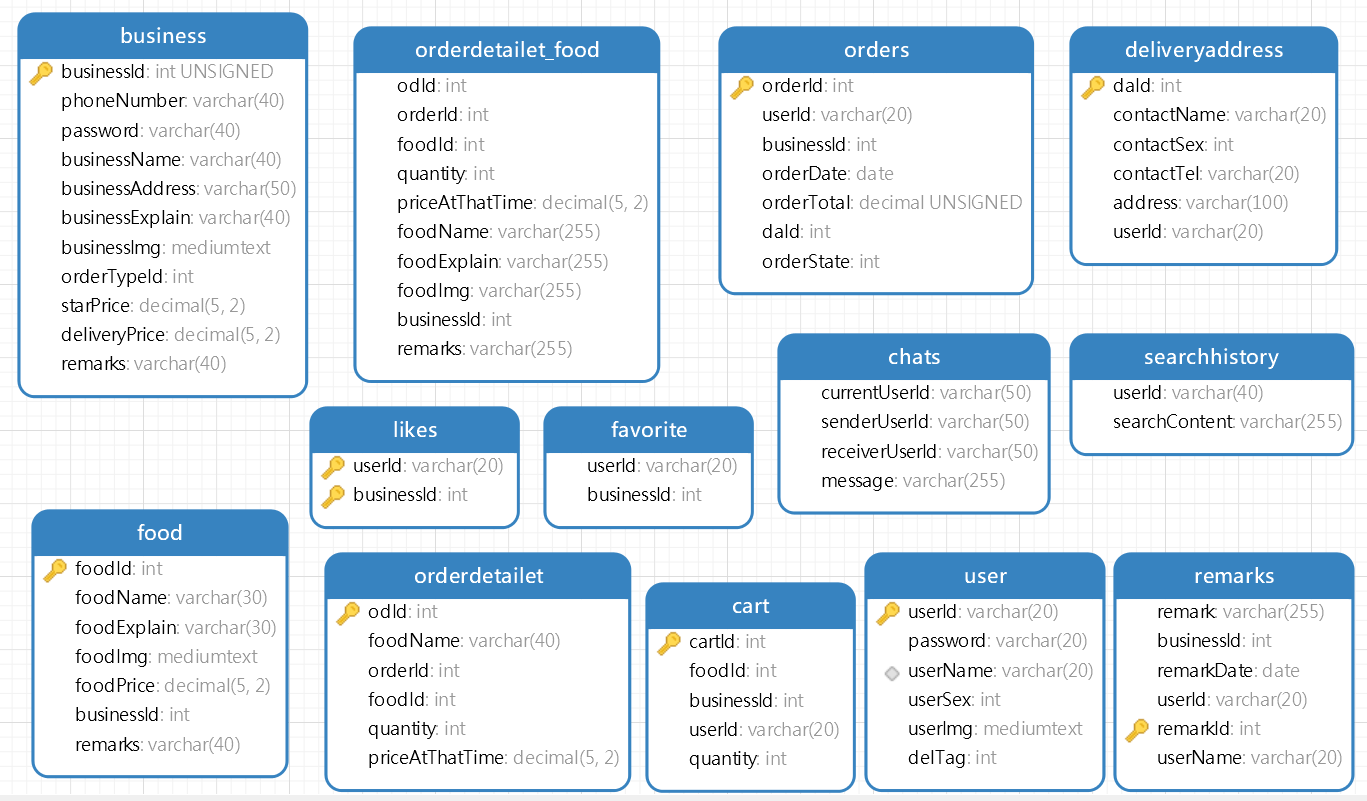
\includegraphics[width=1\textwidth]{Picture20}
  \caption{数据库表结构}\label{fig:xml}
  \vspace{\baselineskip}
\end{figure}



\section{部署的步骤和流程}

\subsection{服务器配置}
\begin{enumerate}
  \item 安装 Ubuntu 20.04 LTS 服务器。
  \item 安装 Nginx 和 MySQL。
  \item 安装 Java 和 Spring Boot。
  \item 安装 Redis 和 RabbitMQ。
\end{enumerate}
\subsection{前端部署}
\begin{enumerate}
  \item 将前端代码部署到服务器上。
  \item 配置 Nginx,将前端请求重定向到服务器。
\end{enumerate}
\subsection{后端部署}
\begin{enumerate}
  \item 将后端代码部署到服务器上。
  \item 配置 Nginx,将后端请求重定向到服务器。
\end{enumerate}
\subsection{数据库部署}
\begin{enumerate}
  \item 将数据库部署到服务器上。
\end{enumerate}
\subsection{其他配置}
\begin{enumerate}
  \item 安装宝塔面板,方便操作
  \item 配置 Nginx,将前端和后端请求重定向到服务器。
  \item 配置日志管理,快速定位问题。
\end{enumerate}
	% !Mode:: "TeX:UTF-8"

\chapter{人员分工及项目进度}

\begin{itemize}
  \item \textbf{人员分工:}
  \begin{itemize}
      \item 杨宇鑫:负责后端与部署
      \item 谢帛洋:负责前端与测试
  \end{itemize}
\end{itemize}

\begin{itemize}
\item \textbf{项目进度:}
\begin{itemize}
    \item 第一周:学习了项目一的内容,复盘了项目一的代码;
    \item 第二周:学习了项目二到项目四的内容,复盘了项目二到项目四的代码,饿了吧V1.0项目复盘完成;
    \item 第三周:创新了原项目,饿了吧V2.0项目完成。
\end{itemize}
\end{itemize}

	
\chapter{项目分析及开发过程}

\section{项目分析}
\subsection{项目一: JDBC}
\textbf{elm\_admin 是饿了么 JDBC 版项目,采用了 JDBC+MySQL 开发,是纯后端的字符界面操作数据库的命令行应用程序。}

\subsubsection{项目技术架构}
- JDK 1.8

- JDBC

- MySQL 数据库

\subsubsection{开发工具}
- STS(spring-tool-suite)

- mysql-5.5.62-winx64

- Navicat Premium 8

\subsubsection{安装部署指南}
\begin{itemize}
  \item 安装 jdk、STS、MySQL
  \item 在 MySQL 数据库中创建数据库 \texttt{elm\_admin},使用数据库脚本 \texttt{elm\_admin.sql} 创建数据库和初始数据。  \item 在 STS 中导入 JavaSE 项目。
  \item 打开 \texttt{com/neusoft/elm/util/DBUtil} 修改数据库密码
  \item 本项目有两个入口:管理员入口、商家入口。
      \begin{itemize}
          \item 运行 \texttt{ElmAdminEntry} 中的 main 函数为管理员入口。
          \item 运行 \texttt{ElmBusinessEntry} 中的 main 函数为商家入口。
      \end{itemize}
\end{itemize}
\subsubsection{整体要求}
1. 项目技术架构

   - JDK8
   
   - JDBC
   
   - MySql
   
2. 开发工具

   - STS(SpringToolSuite4)
   
   - mysql-5.5.62-winx64
   
   - navicat
   
3. 涉及的技术点

   - 封装 JDBC

   - 封装 DAO

   - 领域模型中的实体类
   
   - 增删改查操作

   - 多条件模糊查询

   - JDBC 事务管理
   
   - 表的主外键关系
   

   
\subsection{项目二: Vue3}
\textbf{饿了么前端版项目是采用 HTML、CSS、JavaScript 开发的前端静态网页项目。}

\subsubsection{项目前端技术架构}
- HTML

- CSS

- JavaScript


\subsubsection{开发工具}
- HBuilder

- Chrome 浏览器


\subsubsection{安装部署指南}
- 安装 HBuilder、Chrome

- 将工程导入到 HBuilder 中

- 在 Chrome 浏览器中运行 index.html 文件

- 在 Chrome 浏览器中使用 Toggle device toolbar 模拟手机浏览

\subsubsection{整体要求}
1. 项目技术架构

   - HTML5

   - CSS3

   - JavaScript(ES6 以上)

   
2. 开发工具

   - HBuilder

   - Chrome 浏览器

   
3. 涉及的技术点

   - HTML5 标签的使用

   - CSS3 样式的使用

   - JS 对 DOM 的基本操作

   - DIV+CSS 布局基础

   - 移动端布局基础

   - viewport 设置

   - 弹性布局

   - 边框盒子模型

   - vw 与 vh 的使用

   - 图片按比例自适应

   - CSS3 小图标的使用

   - 第三方字体库的使用



\subsection{项目三: Servlet}

% 仅添加换行
\textbf{饿了么 Servlet 版本}

\subsubsection{项目演示}
- 运行 “饿了么项目”,演示应用程序效果,演示 “点餐业务线” 整体流程。

- 本项目参照 “饿了么官网网页版” 制作。饿了么网页版:http://h5.ele.me/

- 本项目专注于完成点餐业务线功能,“饿了么官网” 中的其它功能暂不涉及。


\subsubsection{项目目标}
- 本项目为课程级贯穿项目中的第三个项目(JDBC项目、前端项目、JavaWeb项目)。

- 本项目完成后,学员将能够使用 Vue + Servlet + AJAX 技术开发前后端分离的 Web 应用程序。

\subsubsection{项目中所涉及到相关知识点}
- AJAX 的使用

- Servlet 的使用

- Session 的使用

- 简单 MVC 封装

- Service 层事务管理

- DAO 层批量操作

- 多对一与一对多的映射

- 服务器端 JSON 数据转换

- VueCLI 的使用

- 多条件模糊查询的使用

- SVN、Git 版本控制工具的使用

\subsubsection{数据库设计}
- 本项目完成后,学员将能够使用 Vue + Servlet + AJAX 技术开发前后端分离的 Web 应用程序。

\subsubsection{整体要求}
1. 项目技术架构

- JDK8

- Servlet

- Tomcat5.5

- MySQL

- Vue
   
2. 开发工具

- HBuilder

- STS(SpringToolSuite4)

- mysql-5.5.62-winx64

- Tomcat8.5
   
3. 涉及的技术点

- AJAX 的使用

- Servlet 的使用

- Session 的使用

- 简单 MVC 封装

   - Service 层事务管理

   - DAO 层批量操作

   - 多对一与一对多的映射

   - 服务器端 JSON 数据转换

   - VueCLI 的使用

   - 多条件模糊查询的使用


\subsection{项目四: SpringBoot}
\textbf{饿了么 SpringBoot 版本}

\subsubsection{整体要求}
1. 项目技术架构

- JDK8

- SpringBoot

- MyBatis

- MySQL

- Vue



2. 开发工具

- HBuilder

- STS(SpringToolSuite4)

- mysql-5.5.62-winx64

- Tomcat8.5

- Maven



3. 涉及的技术点

- AJAX 的使用

- SpringBoot 框架的使用

- MyBatis 框架的使用

- 封装 Mapper

- Service 层事务管理

- 数据层批量操作

- 多对一与一对多的映射

- 服务器端 JSON 数据转换

- VueCLI 的使用

- 多条件模糊查询的使用

\section{开发过程}

\begin{itemize}
    \item \textbf{项目进度:}
    \begin{itemize}
        \item 第一周:学习了项目一的内容,复盘了项目一的代码;
        \item 第二周:学习了项目二到项目四的内容,复盘了项目二到项目四的代码,饿了吧V1.0项目复盘完成,并完成了前后端的部署;
        \item 第三周:创新了原项目,饿了吧V2.0项目完成,前后端数据库都部署在了腾讯云服务器上,并制作了简易的手机apk
    \end{itemize}
\end{itemize}

\section{gitee上团队成员贡献}

\begin{figure}[htbp]
    \centering
    \begin{minipage}{0.4\textwidth}
    \centering
    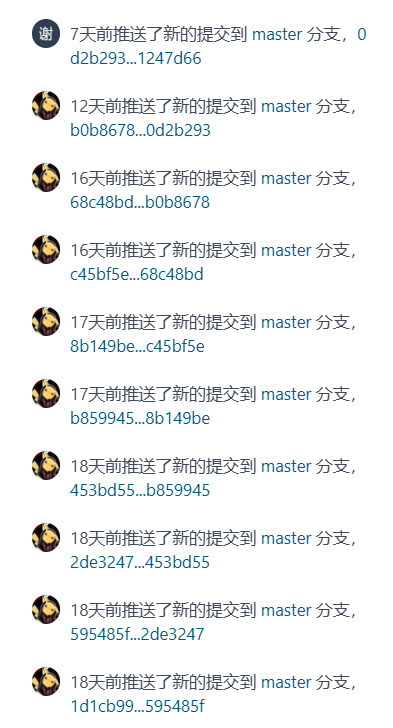
\includegraphics[width=\textwidth]{Picture1}
    \caption{Gitee提交数据1}\label{fig:dd}
    \end{minipage}
    \begin{minipage}{0.4\textwidth}
    \centering
    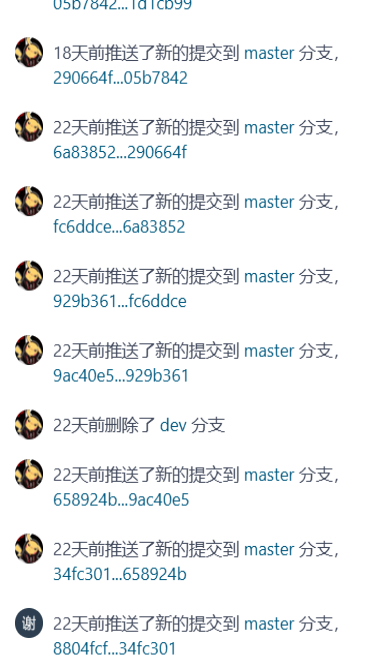
\includegraphics[width=\textwidth]{Picture2}
    \caption{Gitee提交数据2}\label{fig:ds}
    \end{minipage}
    \vspace{\baselineskip}
    \end{figure}

    \begin{figure}[htbp]
        \centering
        \begin{minipage}{0.4\textwidth}
        \centering
        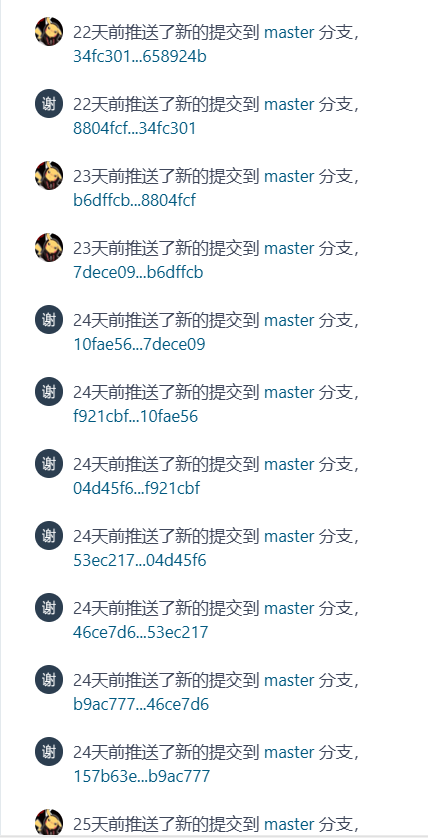
\includegraphics[width=\textwidth]{Picture3}
        \caption{Gitee提交数据3}\label{fig:dd}
        \end{minipage}
        \begin{minipage}{0.4\textwidth}
        \centering
        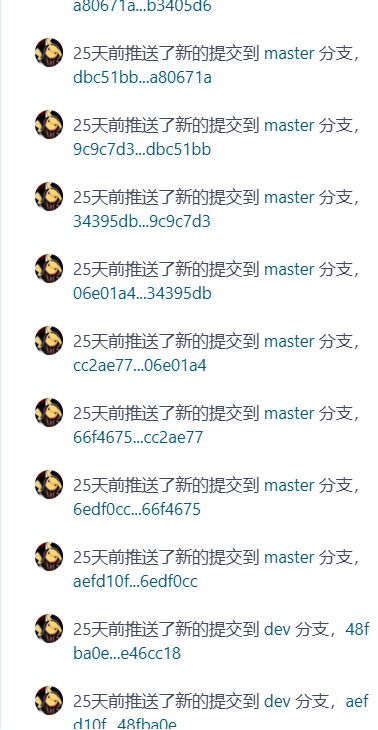
\includegraphics[width=\textwidth]{Picture4}
        \caption{Gitee提交数据4}\label{fig:ds}
        \end{minipage}
        \vspace{\baselineskip}
        \end{figure}

	
\chapter{开发过程}

\section{Bug修复以及简单功能的完善}

\begin{itemize}
  \item \textbf{Bug修复:}
  \begin{itemize}
      \item 修复总价浮点数精度 bug;
      \item 修复页面显示不全的 bug。
  \end{itemize}
  \item \textbf{功能完善:}
  \begin{itemize}
      \item 手机号的正则表达式检验;
      \item 强密码检验。
  \end{itemize}
\end{itemize}


\section{饿了吧V2.0版本的创新点}
% 插入创新点信息

\subsection{实现前端 Vue2 到 Vue3 的升级}

\subsection{实现“我的”页面}

\begin{figure}[H]
\centering
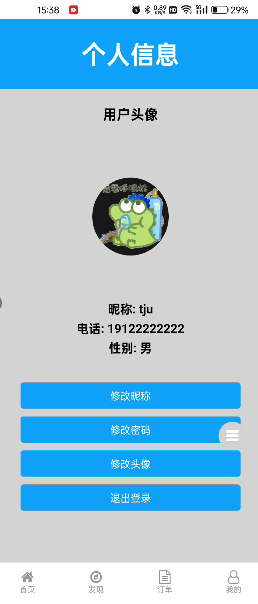
\includegraphics[width=0.4\textwidth]{Picture5}
\caption{实现“我的”页面}\label{fig:xml}
\end{figure}


\subsection{实现修改昵称,修改头像,修改密码功能}

\begin{figure}[H]
  \centering
  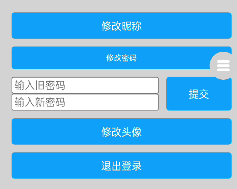
\includegraphics[width=0.4\textwidth]{Pictur6}
  \caption{实现修改昵称,修改头像,修改密码功能}\label{fig:xml}
  \end{figure}

\subsection{实现收藏功能:收藏商家,取消收藏,收藏列表}

\begin{figure}[H]
  \centering
  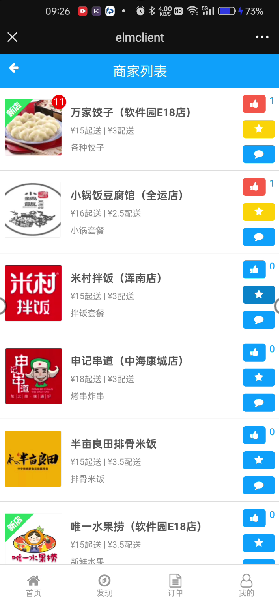
\includegraphics[width=0.4\textwidth]{Picture7}
  \caption{实现收藏功能:收藏商家,取消收藏,收藏列表}\label{fig:xml}
  \end{figure}

\subsection{实现点赞功能:点赞,取消点赞,展示商家总点赞量}

\begin{figure}[H]
  \centering
  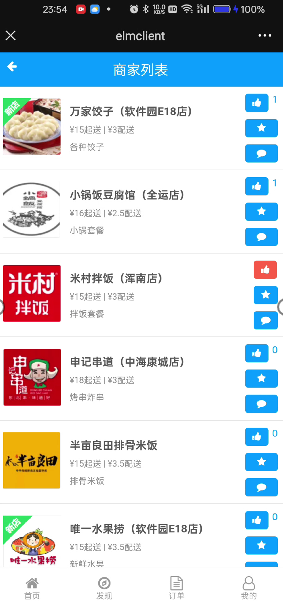
\includegraphics[width=0.4\textwidth]{Picture8}
  \caption{实现点赞功能:点赞,取消点赞,展示商家总点赞量}\label{fig:xml}
  \end{figure}

\subsection{实现评论功能:新增评论,展示评论列表,删除评论}

\begin{figure}[H]
  \centering
  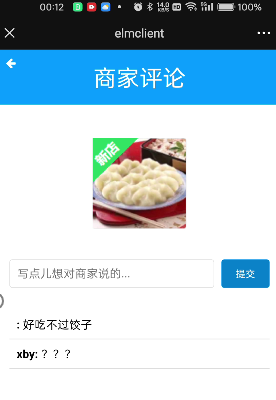
\includegraphics[width=0.4\textwidth]{Pictur9}
  \caption{实现评论功能:新增评论,展示评论列表,删除评论}\label{fig:xml}
  \end{figure}

\subsection{实现搜索功能:模糊匹配,可以搜索商家或商品}

\begin{figure}[H]
  \centering
  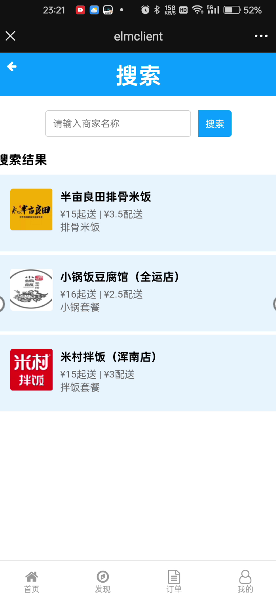
\includegraphics[width=0.4\textwidth]{Picture10}
  \caption{实现搜索功能:模糊匹配,可以搜索商家或商品}\label{fig:xml}
  \end{figure}

\subsection{实现历史记录功能:搜索的时候展示搜索历史}

\begin{figure}[H]
  \centering
  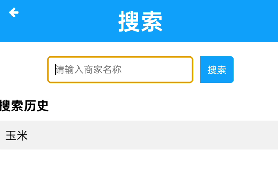
\includegraphics[width=1\textwidth]{Picture11}
  \caption{实现历史记录功能:搜索的时候展示搜索历史}\label{fig:xml}
  \end{figure}

\subsection{实现商家账号注册,登录,上架商品,修改商家个人信息}

\begin{figure}[H]
  \centering
  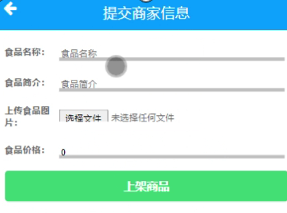
\includegraphics[width=1\textwidth]{Picture12}
  \caption{实现商家账号注册,登录,上架商品,修改商家个人信息}\label{fig:xml}
  \end{figure}

  \subsection{集成文心一言接口,充当智能客服,方便用户对食品的咨询}

  \begin{figure}[H]
  \centering
  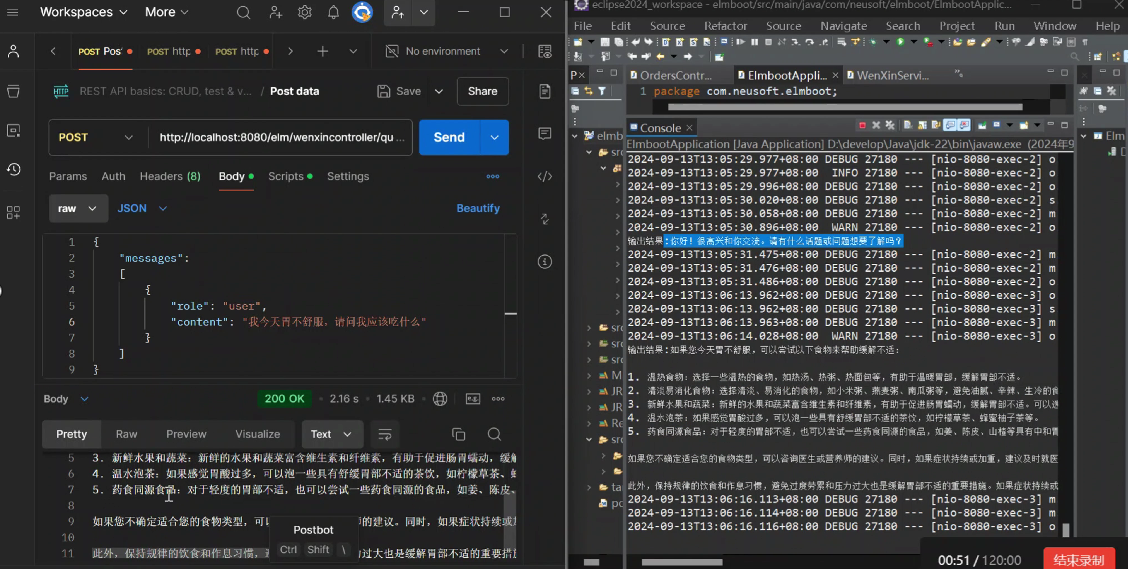
\includegraphics[width=1\textwidth]{Picture13}
  \caption{集成文心一言接口,充当智能客服,方便用户对食品的咨询}\label{fig:xml}
  \end{figure}


\section{部署成果}

\subsection{在腾讯云服务器上部署:前端,后端,数据库}

\begin{figure}[H]
  \centering
  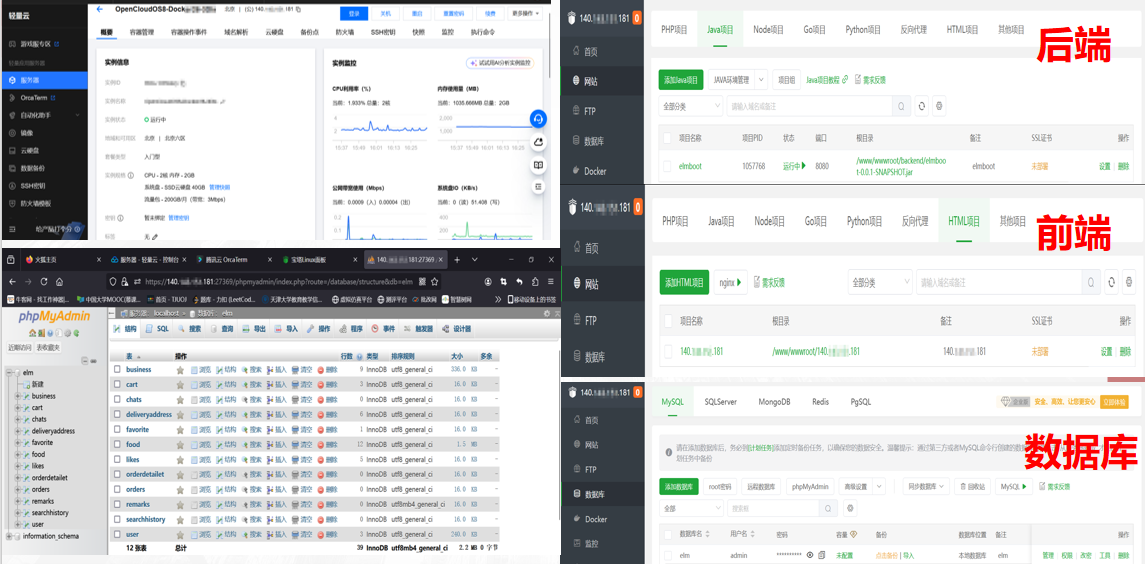
\includegraphics[width=1\textwidth]{Picture14}
  \caption{在腾讯云服务器上部署:前端,后端,数据库}\label{fig:xml}
  \end{figure}
\subsection{创建手机 APK}

\begin{figure}[H]
  \centering
  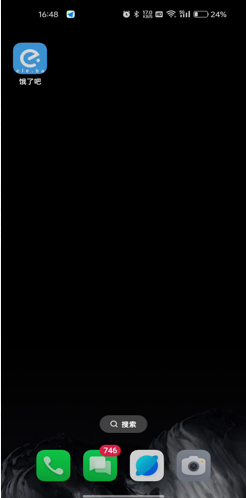
\includegraphics[width=0.4\textwidth]{Picture15}
  \caption{创建手机 APK}\label{fig:xml}
  \end{figure}


	\chapter{问题,解决对策及反思}

\section{浮点数精度}
问题:如果出现3个0.1相加的情况,得到的结果就是0.3000004

解决方案:用字符串表示小数,然后通过字符串相加的算法,得到最终结果

\section{页面显示不全}
问题:有些机型在页面下拉的时候,由于底部有遮挡,没有办法下拉到最下边

解决方案:底部适当留白

反思:站在用户的角度,完善页面布局,给用户最好的体验

\section{历史订单的价格不能随着新的商品价格变化而变化}
问题:当改变数据库一个商品价格的时候,之前已经购买的商品的价格也会变化

解决方案:在原有的订单明细表中,增加一个属性;商品的priceAtThatTime,记住商品在购买时的价格
,当展示订单明细的时候,不用在数据库中去找现在的商品,而是直接在订单明细表中拿到当时的商品价格

反思:当想要保留一个数据的时候,可以直接在数据库中增加属性,在创建的时候,可以直接将值保留进数据库,
在想用的时候直接从数据库中拿到想要的值就可以了


\section{商品详情页的图片不能显示}
问题:商品详情页的图片不能显示,因为图片的url是相对路径,需要将图片的url改为绝对路径

解决方案:在数据库中,将图片的url改为绝对路径,在商品详情页中,通过绝对路径来获取图片

反思:在数据库中,将图片的url改为绝对路径,在商品详情页中,通过绝对路径来获取图片,
这样,在商品详情页中,图片的url就无需再通过服务器来获取了

\section{搜索}
问题:搜索功能,只能搜索到商家,无法搜索到想要的商品

解决方案:强化搜索的sql语句:先将商家与商品按照商家的id进行左连接,并筛选出带有关键词的
商家or商品,将筛选出满足条件的所有商家的id,再显示所有的商家id在(in)刚才筛选出的id中的商家即可

反思:优化sql语句,可以实现更强大的功能

\section{手机号和密码的强度检验}
问题:如果没有检验,用户使用的手机号和密码将会泛滥,失去控制

解决方案:使用正则表达式进行手机号与密码的强度判断

\section{点赞,收藏,评论的存储}

问题:用户的点赞,收藏,评论如何永久保留

解决方案:在数据库中新建点赞,收藏,评论的表结构,并约束好主键外键,设计索引以便更方便的查询数据库中的数据

\section{文心一言的接口}

问题:在javaweb工程中,如何调用文心一言的接口

解决方案:通过查询文心一言api的官网,根据教程与代码,在javaweb工程中,通过HttpClient调用文心一言的接口,并获取返回结果

\section{部署到云端}

问题:如何将本地的javaweb工程部署到云端,并让云端能访问到前端后端以及数据库

解决方案:注册腾讯云账号,开通一个云服务器,因为云服务器上的操作系统是linux,
不方便操作,所以安装宝塔面板,通过数据库部署,html前端部署,java后端部署以及一些配置
完成云端部署,并可以通过公网ip访问到云端的项目
	\chapter{成果与展望}

经过团队成员共同努力,“饿了吧”项目不仅按期完成了既定目标,还超预期地实现了多项创新功能。未来我们将继续关注,不断迭代优化产品,力求提供更加优质的服务。同时,我们也将积极探索新技术的应用,如AI推荐算法等,以期进一步提升平台智能化水平

“饿了吧”项目的成功离不开每一位参与者的辛勤付出与智慧贡献。它不仅是对我们现有技术水平的一次检验,更为重要的是它代表了我们对未来发展方向的一种探索。希望以此为契机,能够激励更多人投身于技术创新之中,共同推动行业进步。

	
	% % !Mode:: "TeX:UTF-8"

\chapter{实践简介}

\section{实践背景}
\begin{enumerate}
\item 学习并学解JDBC、HTML、CSS、JavaScript、Servlet、Springboot等知识。
\item 完成饿了吧项目一、二、三、四的实现。
\end{enumerate}

\section{实践内容}
\begin{enumerate}
\item 完成项目一JDBC版本的实现。
\item 完成项目二HTML+css+js版本的实现。
\item 完成项目三Servlet版本的实现。
\item 完成项目四Springboot版本的实现。
\end{enumerate}

\section{实践目的}
\begin{enumerate}
\item 了解JDBC、HTML、CSS、JavaScript、Servlet、Springboot等知识。
\item 完成饿了吧项目V2.0的实现。
\end{enumerate}


\section{具体要求}

\subsection*{项目一: JDBC}
\textbf{elm\_admin 是饿了么 JDBC 版项目,采用了 JDBC+MySQL 开发,是纯后端的字符界面操作数据库的命令行应用程序。}
\subsubsection*{1. 简介}

\paragraph*{1.1 项目技术架构}
- JDK 1.8
- JDBC
- MySQL 数据库

\paragraph*{1.2 开发工具}
- STS(spring-tool-suite)
- mysql-5.5.62-winx64
- Navicat Premium 8

\subsubsection*{2. 安装部署指南}
\begin{itemize}
  \item 安装 jdk、STS、MySQL
  \item 在 MySQL 数据库中创建数据库 \texttt{elm\_admin},使用数据库脚本 \texttt{elm\_admin.sql} 创建数据库和初始数据。  \item 在 STS 中导入 JavaSE 项目。
  \item 打开 \texttt{com/neusoft/elm/util/DBUtil} 修改数据库密码
  \item 本项目有两个入口:管理员入口、商家入口。
      \begin{itemize}
          \item 运行 \texttt{ElmAdminEntry} 中的 main 函数为管理员入口。
          \item 运行 \texttt{ElmBusinessEntry} 中的 main 函数为商家入口。
      \end{itemize}
\end{itemize}
\subsubsection*{3. 整体要求}
1. 项目技术架构
   - JDK8
   - JDBC
   - MySql
   
2. 开发工具
   - STS(SpringToolSuite4)
   - mysql-5.5.62-winx64
   - navicat
   
3. 涉及的技术点
   - 封装 JDBC
   - 封装 DAO
   - 领域模型中的实体类
   - 增删改查操作
   - 多条件模糊查询
   - JDBC 事务管理
   - 表的主外键关系

   
\subsection*{项目二: Vue3}
\textbf{饿了么前端版项目是采用 HTML、CSS、JavaScript 开发的前端静态网页项目。}

\subsubsection*{1. 简介}

\paragraph*{1.1 项目前端技术架构}
- HTML
- CSS
- JavaScript

\paragraph*{1.2 开发工具}
- HBuilder
- Chrome 浏览器

\subsubsection*{2. 安装部署指南}
- 安装 HBuilder、Chrome
- 将工程导入到 HBuilder 中
- 在 Chrome 浏览器中运行 index.html 文件
- 在 Chrome 浏览器中使用 Toggle device toolbar 模拟手机浏览

\subsubsection*{3. 整体要求}
1. 项目技术架构
   - HTML5
   - CSS3
   - JavaScript(ES6 以上)
   
2. 开发工具
   - HBuilder
   - Chrome 浏览器
   
3. 涉及的技术点
   - HTML5 标签的使用
   - CSS3 样式的使用
   - JS 对 DOM 的基本操作
   - DIV+CSS 布局基础
   - 移动端布局基础
   - viewport 设置
   - 弹性布局
   - 边框盒子模型
   - vw 与 vh 的使用
   - 图片按比例自适应
   - CSS3 小图标的使用
   - 第三方字体库的使用


\subsection*{项目三: Servlet}

% 仅添加换行
\textbf{饿了么 Servlet 版本}

\subsubsection*{1. 项目概述}

\paragraph*{1.1 项目演示}
- 运行 “饿了么项目”,演示应用程序效果,演示 “点餐业务线” 整体流程。
- 本项目参照 “饿了么官网网页版” 制作。饿了么网页版:http://h5.ele.me/
- 本项目专注于完成点餐业务线功能,“饿了么官网” 中的其它功能暂不涉及。

\paragraph*{1.2 项目目标}
- 本项目为课程级贯穿项目中的第三个项目(JDBC项目、前端项目、JavaWeb项目)。
- 本项目完成后,学员将能够使用 Vue + Servlet + AJAX 技术开发前后端分离的 Web 应用程序。

\paragraph*{1.3 项目中所涉及到相关知识点}
- AJAX 的使用
- Servlet 的使用
- Session 的使用
- 简单 MVC 封装
- Service 层事务管理
- DAO 层批量操作
- 多对一与一对多的映射
- 服务器端 JSON 数据转换
- VueCLI 的使用
- 多条件模糊查询的使用
- SVN、Git 版本控制工具的使用

\paragraph*{1.4 数据库设计}
- 本项目完成后,学员将能够使用 Vue + Servlet + AJAX 技术开发前后端分离的 Web 应用程序。

\subsubsection*{1.5 整体要求}
1. 项目技术架构
   - JDK8
   - Servlet
   - Tomcat5.5
   - MySQL
   - Vue
   
2. 开发工具
   - HBuilder
   - STS(SpringToolSuite4)
   - mysql-5.5.62-winx64
   - Tomcat8.5
   
3. 涉及的技术点
   - AJAX 的使用
   - Servlet 的使用
   - Session 的使用
   - 简单 MVC 封装
   - Service 层事务管理
   - DAO 层批量操作
   - 多对一与一对多的映射
   - 服务器端 JSON 数据转换
   - VueCLI 的使用
   - 多条件模糊查询的使用


\subsection*{项目四: SpringBoot}
\textbf{饿了么 SpringBoot 版本}

\subsubsection*{1. 整体要求}
1. 项目技术架构
   - JDK8
   - SpringBoot
   - MyBatis
   - MySQL
   - Vue
   
2. 开发工具
   - HBuilder
   - STS(SpringToolSuite4)
   - mysql-5.5.62-winx64
   - Tomcat8.5
   - Maven
   
3. 涉及的技术点
   - AJAX 的使用
   - SpringBoot 框架的使用
   - MyBatis 框架的使用
   - 封装 Mapper
   - Service 层事务管理
   - 数据层批量操作
   - 多对一与一对多的映射
   - 服务器端 JSON 数据转换
   - VueCLI 的使用
   - 多条件模糊查询的使用
	% 
\chapter{项目分析及开发过程}

\section{项目分析}
\subsection{项目一: JDBC}
\textbf{elm\_admin 是饿了么 JDBC 版项目,采用了 JDBC+MySQL 开发,是纯后端的字符界面操作数据库的命令行应用程序。}

\subsubsection{项目技术架构}
- JDK 1.8

- JDBC

- MySQL 数据库

\subsubsection{开发工具}
- STS(spring-tool-suite)

- mysql-5.5.62-winx64

- Navicat Premium 8

\subsubsection{安装部署指南}
\begin{itemize}
  \item 安装 jdk、STS、MySQL
  \item 在 MySQL 数据库中创建数据库 \texttt{elm\_admin},使用数据库脚本 \texttt{elm\_admin.sql} 创建数据库和初始数据。  \item 在 STS 中导入 JavaSE 项目。
  \item 打开 \texttt{com/neusoft/elm/util/DBUtil} 修改数据库密码
  \item 本项目有两个入口:管理员入口、商家入口。
      \begin{itemize}
          \item 运行 \texttt{ElmAdminEntry} 中的 main 函数为管理员入口。
          \item 运行 \texttt{ElmBusinessEntry} 中的 main 函数为商家入口。
      \end{itemize}
\end{itemize}
\subsubsection{整体要求}
1. 项目技术架构

   - JDK8
   
   - JDBC
   
   - MySql
   
2. 开发工具

   - STS(SpringToolSuite4)
   
   - mysql-5.5.62-winx64
   
   - navicat
   
3. 涉及的技术点

   - 封装 JDBC

   - 封装 DAO

   - 领域模型中的实体类
   
   - 增删改查操作

   - 多条件模糊查询

   - JDBC 事务管理
   
   - 表的主外键关系
   

   
\subsection{项目二: Vue3}
\textbf{饿了么前端版项目是采用 HTML、CSS、JavaScript 开发的前端静态网页项目。}

\subsubsection{项目前端技术架构}
- HTML

- CSS

- JavaScript


\subsubsection{开发工具}
- HBuilder

- Chrome 浏览器


\subsubsection{安装部署指南}
- 安装 HBuilder、Chrome

- 将工程导入到 HBuilder 中

- 在 Chrome 浏览器中运行 index.html 文件

- 在 Chrome 浏览器中使用 Toggle device toolbar 模拟手机浏览

\subsubsection{整体要求}
1. 项目技术架构

   - HTML5

   - CSS3

   - JavaScript(ES6 以上)

   
2. 开发工具

   - HBuilder

   - Chrome 浏览器

   
3. 涉及的技术点

   - HTML5 标签的使用

   - CSS3 样式的使用

   - JS 对 DOM 的基本操作

   - DIV+CSS 布局基础

   - 移动端布局基础

   - viewport 设置

   - 弹性布局

   - 边框盒子模型

   - vw 与 vh 的使用

   - 图片按比例自适应

   - CSS3 小图标的使用

   - 第三方字体库的使用



\subsection{项目三: Servlet}

% 仅添加换行
\textbf{饿了么 Servlet 版本}

\subsubsection{项目演示}
- 运行 “饿了么项目”,演示应用程序效果,演示 “点餐业务线” 整体流程。

- 本项目参照 “饿了么官网网页版” 制作。饿了么网页版:http://h5.ele.me/

- 本项目专注于完成点餐业务线功能,“饿了么官网” 中的其它功能暂不涉及。


\subsubsection{项目目标}
- 本项目为课程级贯穿项目中的第三个项目(JDBC项目、前端项目、JavaWeb项目)。

- 本项目完成后,学员将能够使用 Vue + Servlet + AJAX 技术开发前后端分离的 Web 应用程序。

\subsubsection{项目中所涉及到相关知识点}
- AJAX 的使用

- Servlet 的使用

- Session 的使用

- 简单 MVC 封装

- Service 层事务管理

- DAO 层批量操作

- 多对一与一对多的映射

- 服务器端 JSON 数据转换

- VueCLI 的使用

- 多条件模糊查询的使用

- SVN、Git 版本控制工具的使用

\subsubsection{数据库设计}
- 本项目完成后,学员将能够使用 Vue + Servlet + AJAX 技术开发前后端分离的 Web 应用程序。

\subsubsection{整体要求}
1. 项目技术架构

- JDK8

- Servlet

- Tomcat5.5

- MySQL

- Vue
   
2. 开发工具

- HBuilder

- STS(SpringToolSuite4)

- mysql-5.5.62-winx64

- Tomcat8.5
   
3. 涉及的技术点

- AJAX 的使用

- Servlet 的使用

- Session 的使用

- 简单 MVC 封装

   - Service 层事务管理

   - DAO 层批量操作

   - 多对一与一对多的映射

   - 服务器端 JSON 数据转换

   - VueCLI 的使用

   - 多条件模糊查询的使用


\subsection{项目四: SpringBoot}
\textbf{饿了么 SpringBoot 版本}

\subsubsection{整体要求}
1. 项目技术架构

- JDK8

- SpringBoot

- MyBatis

- MySQL

- Vue



2. 开发工具

- HBuilder

- STS(SpringToolSuite4)

- mysql-5.5.62-winx64

- Tomcat8.5

- Maven



3. 涉及的技术点

- AJAX 的使用

- SpringBoot 框架的使用

- MyBatis 框架的使用

- 封装 Mapper

- Service 层事务管理

- 数据层批量操作

- 多对一与一对多的映射

- 服务器端 JSON 数据转换

- VueCLI 的使用

- 多条件模糊查询的使用

\section{开发过程}

\begin{itemize}
    \item \textbf{项目进度:}
    \begin{itemize}
        \item 第一周:学习了项目一的内容,复盘了项目一的代码;
        \item 第二周:学习了项目二到项目四的内容,复盘了项目二到项目四的代码,饿了吧V1.0项目复盘完成,并完成了前后端的部署;
        \item 第三周:创新了原项目,饿了吧V2.0项目完成,前后端数据库都部署在了腾讯云服务器上,并制作了简易的手机apk
    \end{itemize}
\end{itemize}

\section{gitee上团队成员贡献}

\begin{figure}[htbp]
    \centering
    \begin{minipage}{0.4\textwidth}
    \centering
    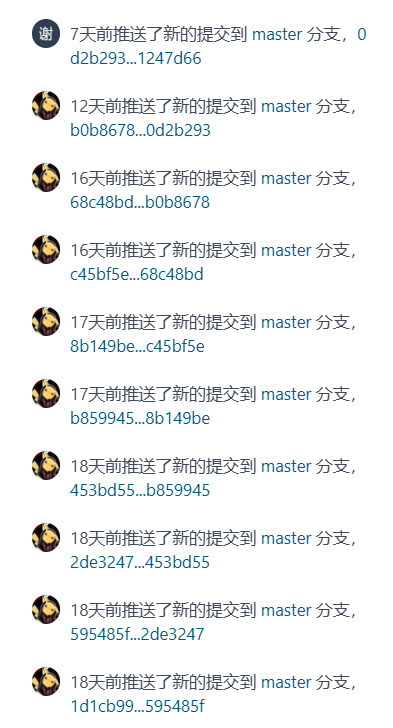
\includegraphics[width=\textwidth]{Picture1}
    \caption{Gitee提交数据1}\label{fig:dd}
    \end{minipage}
    \begin{minipage}{0.4\textwidth}
    \centering
    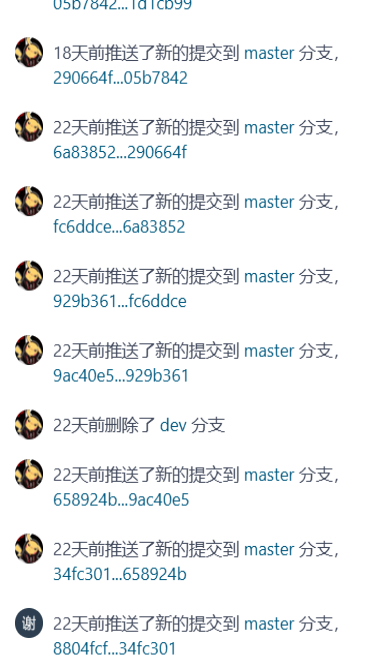
\includegraphics[width=\textwidth]{Picture2}
    \caption{Gitee提交数据2}\label{fig:ds}
    \end{minipage}
    \vspace{\baselineskip}
    \end{figure}

    \begin{figure}[htbp]
        \centering
        \begin{minipage}{0.4\textwidth}
        \centering
        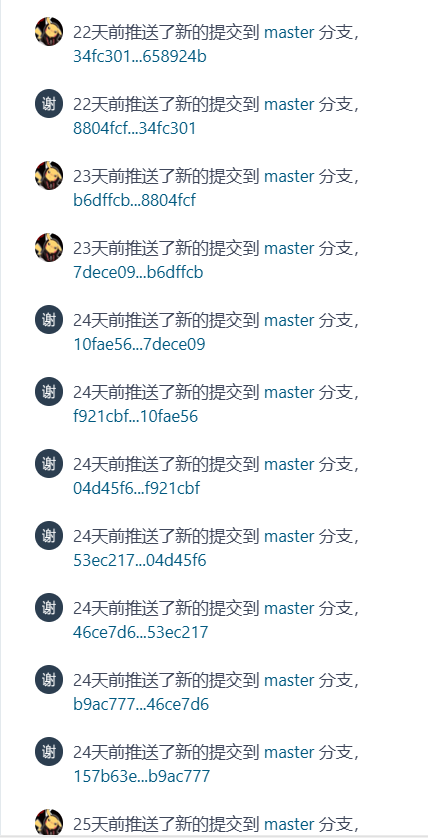
\includegraphics[width=\textwidth]{Picture3}
        \caption{Gitee提交数据3}\label{fig:dd}
        \end{minipage}
        \begin{minipage}{0.4\textwidth}
        \centering
        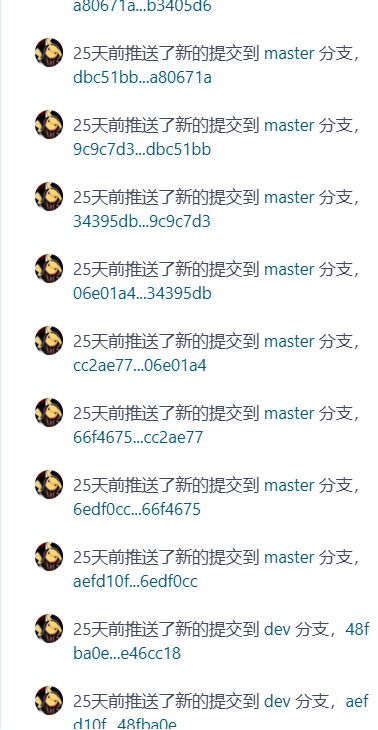
\includegraphics[width=\textwidth]{Picture4}
        \caption{Gitee提交数据4}\label{fig:ds}
        \end{minipage}
        \vspace{\baselineskip}
        \end{figure}

	% % !Mode:: "TeX:UTF-8"

\chapter{实践成果}




\end{CJK*}                                     % 结束中文字体使用
\end{document}                                 % 结束全文
